\documentclass[a4paper,14pt]{extreport}

% Кодировка и язык
\usepackage[utf8]{inputenc}
\usepackage[T2A]{fontenc}
\usepackage[english,russian]{babel}

% Поля страницы
\usepackage[left=2.5cm,right=1.5cm,top=2cm,bottom=2cm]{geometry}

% Графика и изображения
\usepackage{graphicx}
\usepackage{float}
\usepackage{subcaption}
\usepackage{xcolor}

% Математика и формулы
\usepackage{amsmath}
\usepackage{amssymb}
\usepackage{amsfonts}

% Таблицы
\usepackage{array}
\usepackage{tabularx}
\usepackage{longtable}
\usepackage{booktabs}
\usepackage{multirow}
\usepackage{colortbl}

% Гиперссылки
\usepackage[colorlinks=true,linkcolor=blue,citecolor=blue,urlcolor=blue]{hyperref}

% Листинги кода
\usepackage{listings}
\usepackage{courier}

% Заголовки
\usepackage{titlesec}
\usepackage{tocloft}

% Интервалы
\usepackage{setspace}
\onehalfspacing

% Оформление заголовков
\titleformat{\chapter}[display]
  {\normalfont\huge\bfseries}{\chaptertitlename\ \thechapter}{20pt}{\Huge}
\titleformat{\section}
  {\normalfont\Large\bfseries}{\thesection}{1em}{}
\titleformat{\subsection}
  {\normalfont\large\bfseries}{\thesubsection}{1em}{}

% Настройка листингов
\lstset{
    basicstyle=\ttfamily\small,
    keywordstyle=\color{blue},
    commentstyle=\color{green!60!black},
    stringstyle=\color{red},
    showstringspaces=false,
    breaklines=true,
    frame=single,
    numbers=left,
    numberstyle=\tiny\color{gray},
    captionpos=b,
    language=Python
}

% Русские названия для элементов
\renewcommand{\contentsname}{Содержание}
\renewcommand{\figurename}{Рисунок}
\renewcommand{\tablename}{Таблица}
\renewcommand{\chaptername}{Глава}
\renewcommand{\appendixname}{Приложение}
\renewcommand{\bibname}{Список литературы}
\renewcommand{\abstractname}{Аннотация}

% Цвета для таблиц
\definecolor{lightgreen}{rgb}{0.9,1,0.9}
\definecolor{lightyellow}{rgb}{1,1,0.9}
\definecolor{lightred}{rgb}{1,0.9,0.9}

% Начало документа
\begin{document}

% Титульный лист
\begin{titlepage}
    \centering
    \vspace*{1cm}
    
    {\Huge\bfseries Исследование методов шифрования\\ в блокчейн-системе Hyperledger Fabric\par}
    
    \vspace{2cm}
    
    {\Large Для дипломной работы\par}
    
    \vspace{3cm}
    
    {\large\itshape Специальность: Информационная безопасность\\
    Направление: Блокчейн-технологии и криптография\par}
    
    \vfill
    
    {\large Автор исследования\par}
    
    \vspace{1cm}
    
    {\large 2024\par}
    
    \vfill
\end{titlepage}

% Аннотация
\begin{abstract}
Данный документ представляет собой исследование криптографических методов и механизмов шифрования, применяемых в разработанной блокчейн-системе на базе Hyperledger Fabric для управления задачами и документами с интеграцией IPFS.

В работе проведён анализ архитектуры криптографической защиты Hyperledger Fabric, изучены используемые алгоритмы цифровой подписи (ECDSA P-256), хеширования (SHA-256) и симметричного шифрования (AES-GCM). Выполнена оценка безопасности текущей реализации системы, выявлены области для улучшения, включая отсутствие шифрования документов в IPFS.

Разработаны практические рекомендации по усилению защиты данных, предложена архитектура гибридного шифрования для IPFS на основе AES-256-GCM, рассмотрены перспективы миграции на постквантовые алгоритмы криптографии.

Исследование сопровождается визуализацией данных в виде 8 профессиональных графиков, демонстрирующих производительность алгоритмов, уровни стойкости, матрицу угроз и архитектуру многоуровневой системы защиты.

\textbf{Ключевые слова:} блокчейн, Hyperledger Fabric, криптография, ECDSA, SHA-256, AES-GCM, IPFS, TLS, постквантовая криптография, информационная безопасность.
\end{abstract}

\tableofcontents
\newpage

% Глава 1: Введение
\chapter{Введение}

\section{Актуальность темы}

В условиях роста требований к безопасности данных и необходимости обеспечения доверия между участниками бизнес-процессов, блокчейн-технологии становятся ключевым инструментом для создания защищённых распределённых систем. Криптографические методы лежат в основе безопасности таких систем, обеспечивая:

\begin{itemize}
    \item \textbf{Конфиденциальность} данных --- защита информации от несанкционированного доступа;
    \item \textbf{Целостность} транзакций --- гарантия неизменности записанных данных;
    \item \textbf{Аутентификацию} участников --- подтверждение идентичности сторон;
    \item \textbf{Неотрекаемость} (non-repudiation) действий --- невозможность отказа от совершенных операций.
\end{itemize}

Hyperledger Fabric как платформа для корпоративных блокчейн-решений предоставляет гибкие механизмы криптографической защиты, однако их эффективное применение требует глубокого понимания архитектурных особенностей и правильных настроек параметров безопасности.

\section{Цель исследования}

Провести анализ криптографических методов, применяемых в блокчейн-системе Hyperledger Fabric, и оценить их эффективность для защиты данных в системе управления задачами и документами.

\section{Задачи исследования}

\begin{enumerate}
    \item Изучить архитектуру криптографической защиты Hyperledger Fabric;
    \item Проанализировать используемые алгоритмы шифрования и хеширования;
    \item Оценить безопасность текущей реализации системы;
    \item Разработать рекомендации по усилению защиты данных;
    \item Создать визуализацию данных для наглядного представления результатов анализа.
\end{enumerate}

\section{Объект и предмет исследования}

\textbf{Объект исследования:} блокчейн-система на базе Hyperledger Fabric для управления задачами и документами с интеграцией IPFS.

\textbf{Предмет исследования:} криптографические методы и механизмы шифрования, применяемые для защиты данных в блокчейн-системе.

\newpage

% Глава 2: Архитектура системы
\chapter{Архитектура системы}

\section{Компоненты системы}

Разработанная система состоит из следующих основных компонентов:

\begin{enumerate}
    \item \textbf{Hyperledger Fabric Network} --- блокчейн-сеть с двумя организациями (Org1, Org2);
    \item \textbf{Chaincode (Smart Contract)} --- смарт-контракт на TypeScript для управления задачами;
    \item \textbf{IPFS Module} --- модуль децентрализованного хранения документов;
    \item \textbf{Backend API} --- REST API на FastAPI с системой ролей;
    \item \textbf{Wallet System} --- система управления идентификационными данными.
\end{enumerate}

\section{Схема потока данных}

На рисунке~\ref{fig:dataflow} представлена схема потока данных в системе.

\begin{figure}[H]
    \centering
    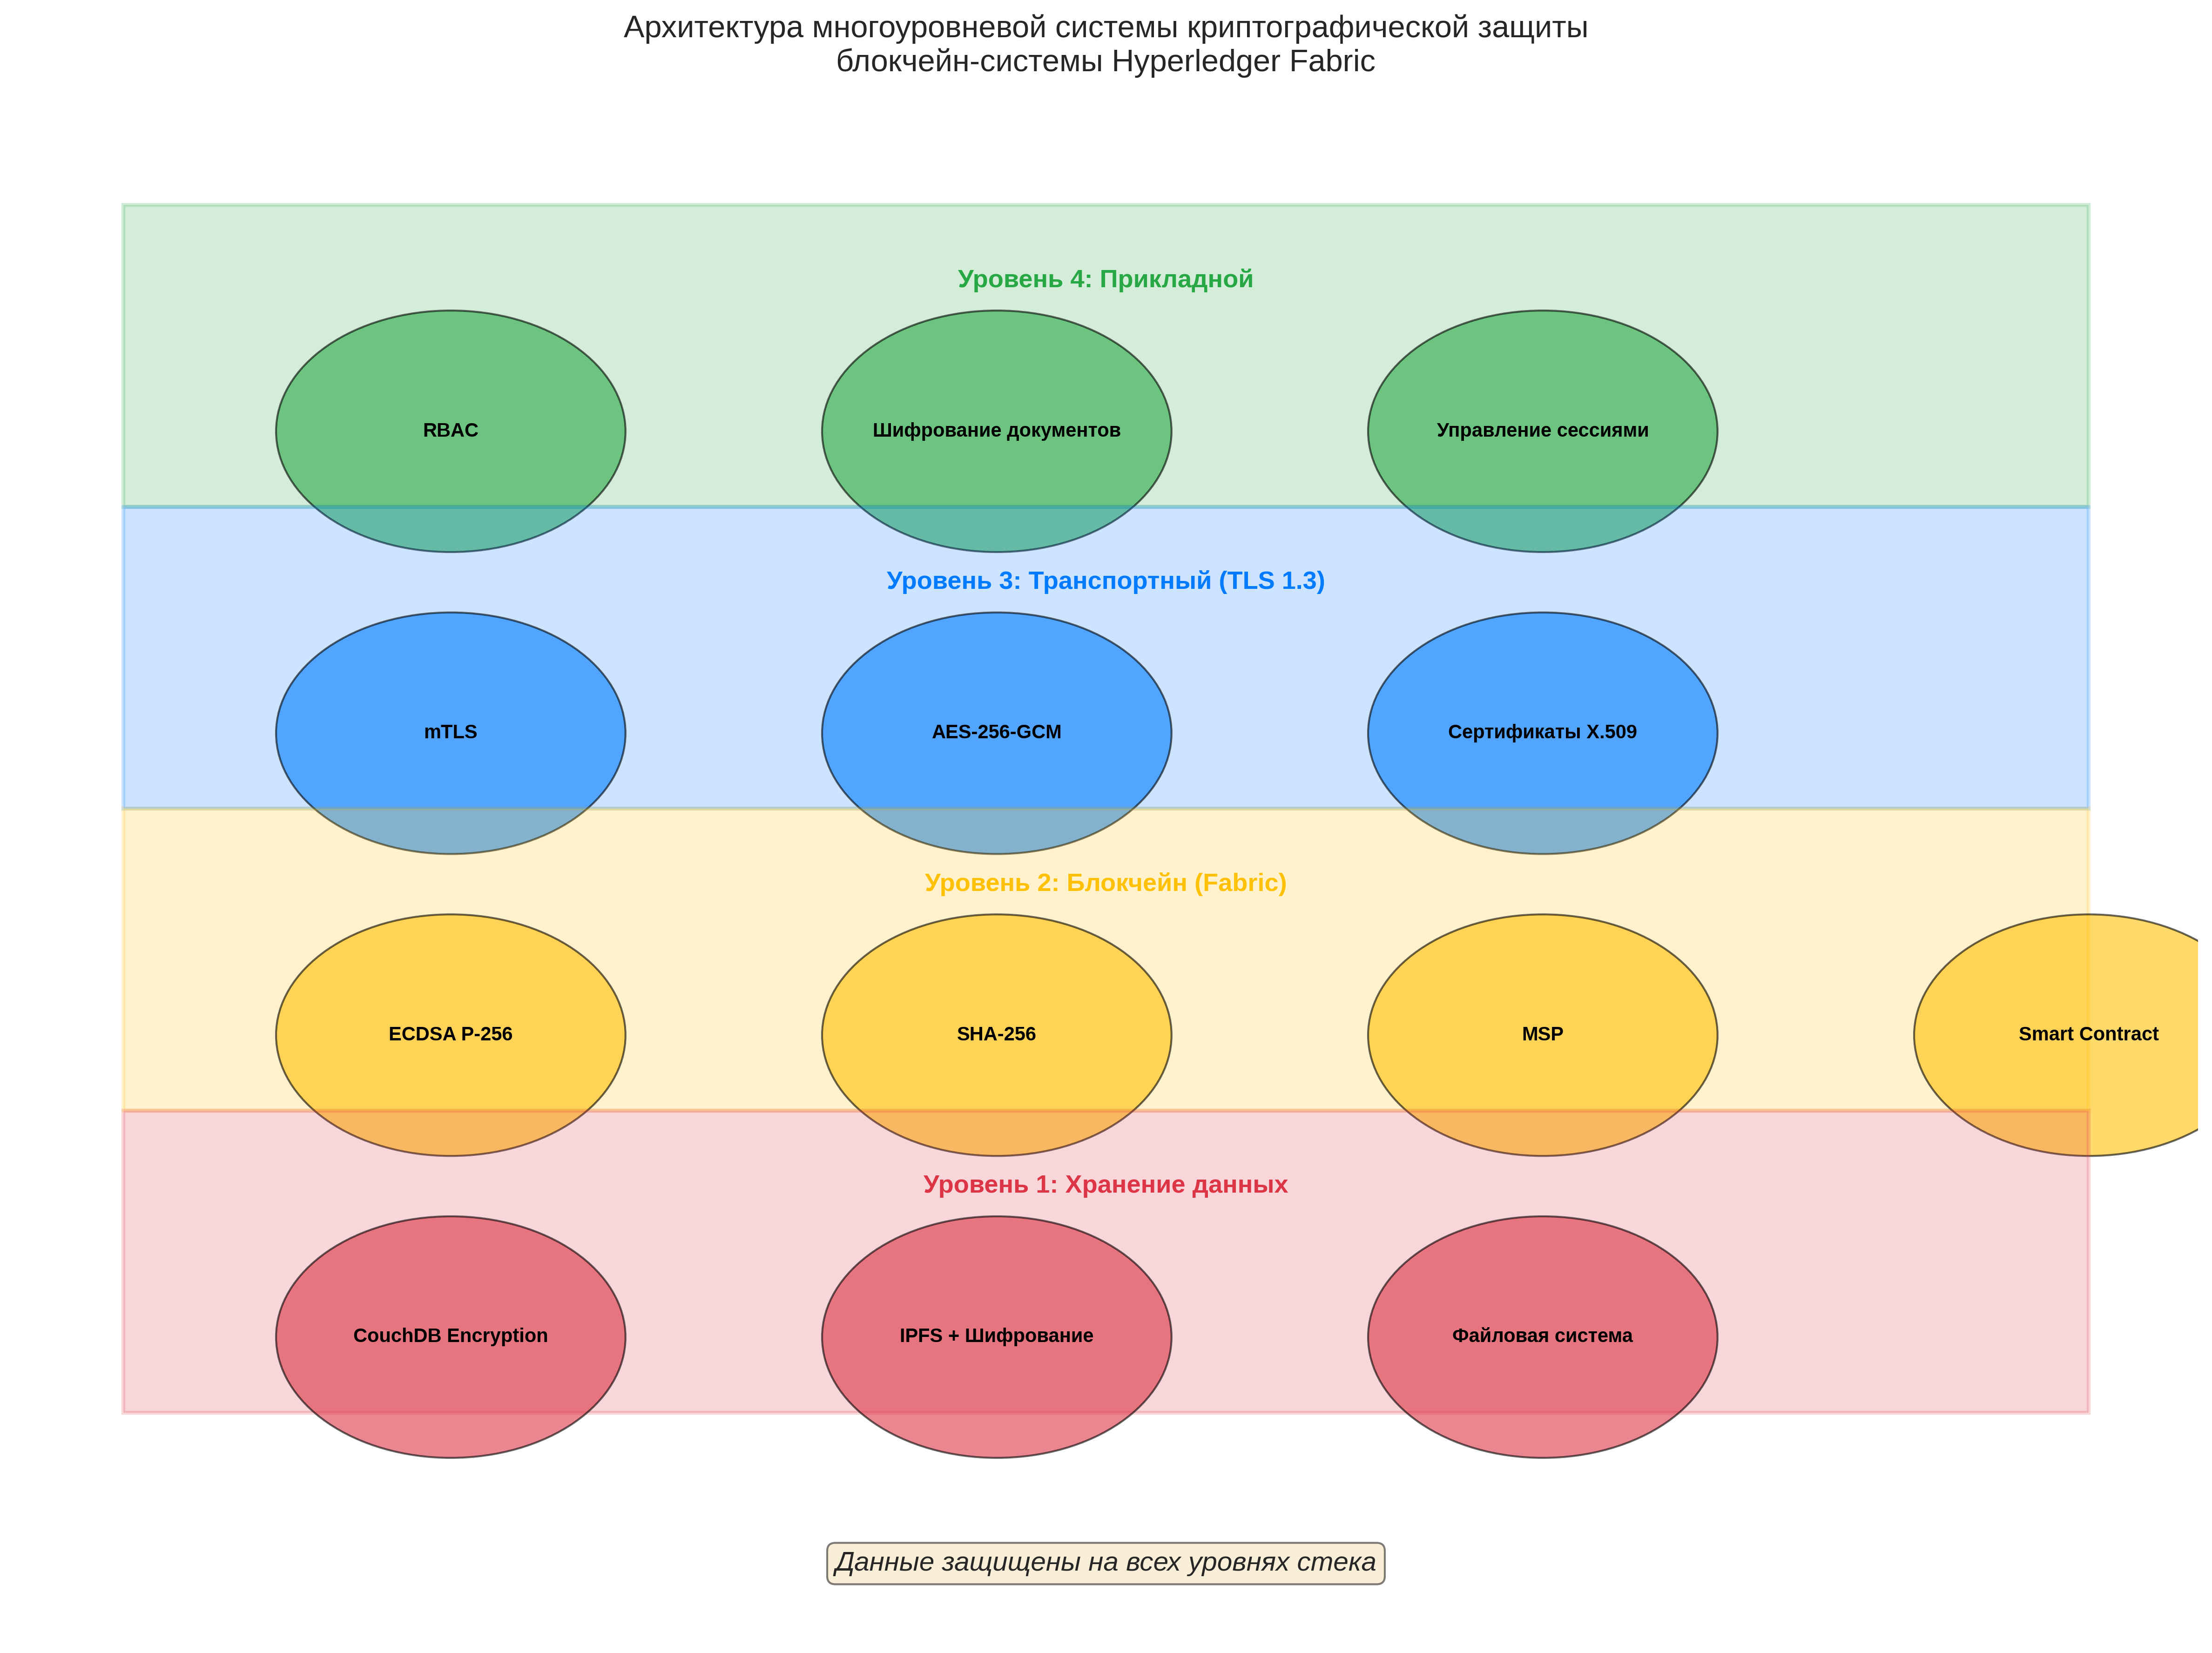
\includegraphics[width=0.9\textwidth]{crypto_charts/architecture_diagram.png}
    \caption{Схема потока данных в блокчейн-системе}
    \label{fig:dataflow}
    \source{Составлено автором}
\end{figure}

Поток данных осуществляется следующим образом:
\begin{enumerate}
    \item Клиентское приложение (Frontend) отправляет запросы через Backend API;
    \item Backend API взаимодействует с сетью Fabric для записи транзакций;
    \item Документы хранятся в IPFS, а их хеши фиксируются в блокчейне;
    \item Состояние блокчейна сохраняется в CouchDB.
\end{enumerate}

\newpage

% Глава 3: Криптографические основы
\chapter{Криптографические основы Hyperledger Fabric}

\section{Инфраструктура открытых ключей (PKI)}

Hyperledger Fabric использует инфраструктуру открытых ключей (Public Key Infrastructure --- PKI) для управления идентификацией участников сети.

\subsection{Компоненты PKI}

\begin{itemize}
    \item \textbf{Fabric CA (Certificate Authority)} --- центр сертификации;
    \item \textbf{X.509 сертификаты} --- цифровые сертификаты стандарта X.509;
    \item \textbf{MSP (Membership Service Provider)} --- поставщик услуг членства.
\end{itemize}

\subsection{Процесс генерации криптографических материалов}

Для генерации криптографических материалов используется утилита \texttt{cryptogen}, которая создаёт:
\begin{itemize}
    \item Сертификаты для организаций (Org1, Org2);
    \item Сертификаты для узлов (peers, orderers);
    \item Сертификаты для пользователей (Admin, User);
    \item Приватные ключи для подписи транзакций.
\end{itemize}

Структура хранилища криптографических материалов:
\begin{verbatim}
organizations/
├── peerOrganizations/
│   └── org1.example.com/
│       ├── peers/
│       │   └── peer0.org1.example.com/
│       │       └── msp/
│       │           ├── keystore/      # Приватные ключи
│       │           ├── signcerts/     # Публичные сертификаты
│       │           └── cacerts/       # Корневые сертификаты
│       └── users/
│           └── Admin@org1.example.com/
│               └── msp/
\end{verbatim}

\section{Алгоритмы цифровой подписи}

\subsection{ECDSA (Elliptic Curve Digital Signature Algorithm)}

Hyperledger Fabric использует ECDSA с кривой \textbf{P-256 (secp256r1)} для подписи транзакций.

\textbf{Характеристики:}
\begin{itemize}
    \item Размер ключа: 256 бит;
    \item Размер подписи: 512 бит (64 байта);
    \item Стойкость: эквивалентна 128 бит симметричного шифрования.
\end{itemize}

\textbf{Процесс подписания транзакции:}
\begin{enumerate}
    \item Клиент создаёт предложение транзакции (transaction proposal);
    \item Вычисляется хеш предложения с использованием SHA-256;
    \item Хеш подписывается приватным ключом клиента с помощью ECDSA;
    \item Подпись прикрепляется к транзакции.
\end{enumerate}

\section{Алгоритмы хеширования}

\subsection{SHA-256 (Secure Hash Algorithm)}

Основной алгоритм хеширования в Fabric.

\textbf{Применение:}
\begin{itemize}
    \item Вычисление идентификаторов транзакций;
    \item Создание хешей блоков;
    \item Генерация идентификаторов состояния (state keys);
    \item Верификация целостности данных.
\end{itemize}

\textbf{Характеристики:}
\begin{itemize}
    \item Размер выхода: 256 бит (32 байта);
    \item Стойкость к коллизиям: $2^{128}$ операций;
    \item Односторонняя функция.
\end{itemize}

\subsection{Хеширование в IPFS}

IPFS использует \textbf{CID (Content Identifier)} на основе хешей:
\begin{itemize}
    \item \textbf{SHA-256} --- основной алгоритм (CID v0);
    \item \textbf{SHA3-256}, \textbf{BLAKE2b} --- поддерживаются в CID v1.
\end{itemize}

\newpage

% Глава 4: Методы шифрования
\chapter{Методы шифрования в системе}

\section{Шифрование каналов связи (TLS)}

\subsection{TLS 1.2/1.3 для защиты коммуникаций}

Все коммуникации в сети Fabric защищены с помощью TLS.

\textbf{Компоненты:}
\begin{itemize}
    \item \textbf{mTLS (mutual TLS)} --- взаимная аутентификация сторон;
    \item \textbf{Сертификаты TLS} --- для каждого компонента сети;
    \item \textbf{Шифрование трафика} --- AES-GCM или ChaCha20-Poly1305.
\end{itemize}

\textbf{Настройка в системе:}
\begin{lstlisting}[language=YAML,caption=Конфигурация Node OU,captionpos=b]
PeerOrgs:
- Name: Org1
  Domain: org1.example.com
  EnableNodeOUs: true  # Включает поддержку Node OU
\end{lstlisting}

\section{Шифрование данных в покое}

\subsection{Уровень базы данных (CouchDB)}

Hyperledger Fabric использует CouchDB как базу данных состояния.

\textbf{Методы защиты:}
\begin{itemize}
    \item Шифрование на уровне файловой системы;
    \item Шифрование на уровне базы данных;
    \item Контроль доступа на уровне документов.
\end{itemize}

\textbf{Рекомендуемая конфигурация:}
\begin{lstlisting}[language=YAML,caption=Конфигурация CouchDB,captionpos=b]
couchdb:
  environment:
    - COUCHDB_USER=admin
    - COUCHDB_PASSWORD=secure_password
  volumes:
    - couchdb_data:/opt/couchdb/data
\end{lstlisting}

\section{Шифрование приватных ключей}

Приватные ключи в Fabric хранятся в зашифрованном виде с использованием защищённых хранилищ операционной системы или аппаратных модулей безопасности (HSM).

\section{Шифрование в IPFS}

\subsection{Проблема публичности данных в IPFS}

IPFS по умолчанию хранит данные в открытом виде. Для защиты конфиденциальных документов применяются следующие методы:

\textbf{Метод 1: Шифрование перед загрузкой}

Использование симметричных алгоритмов шифрования (AES-256-GCM) для шифрования документов перед загрузкой в IPFS.

\textbf{Метод 2: Использование IPFS Encrypted Filesystem (IPFE)}

Шифрование на уровне файловых систем с управлением ключами доступа.

\textbf{Метод 3: Приватные IPFS кластеры}

Изоляция сети IPFS с контролем доступа на уровне сети.

\section{Контроль доступа (RBAC)}

\subsection{Система ролей в backend}

Система реализует Role-Based Access Control со следующими ролями:

\begin{table}[H]
\centering
\caption{Маппинг ролей на разрешения}
\label{tab:roles}
\begin{tabular}{|l|l|}
\hline
\textbf{Роль} & \textbf{Разрешения} \\
\hline
Юрист & add\_document\_version, view\_task, view\_documents \\
Эксперт & confirm\_task, view\_task, view\_documents \\
Модератор & update\_task\_status, view\_task, view\_documents \\
Admin & Все разрешения \\
\hline
\end{tabular}
\end{table}

\newpage

% Глава 5: Анализ безопасности
\chapter{Анализ безопасности}

\section{Угрозы и уязвимости}

\subsection{Категории угроз}

\begin{enumerate}
    \item \textbf{Угрозы конфиденциальности:}
    \begin{itemize}
        \item Перехват незашифрованных данных;
        \item Доступ к приватным ключам;
        \item Утечка данных из IPFS.
    \end{itemize}
    
    \item \textbf{Угрозы целостности:}
    \begin{itemize}
        \item Модификация транзакций;
        \item Подделка подписей;
        \item Атаки 51\% (для Fabric менее актуальны).
    \end{itemize}
    
    \item \textbf{Угрозы доступности:}
    \begin{itemize}
        \item DDoS-атаки;
        \item Отказ оборудования;
        \item Потеря ключей доступа.
    \end{itemize}
\end{enumerate}

\section{Меры противодействия}

\begin{table}[H]
\centering
\caption{Меры противодействия угрозам}
\label{tab:countermeasures}
\begin{tabular}{|l|l|l|}
\hline
\textbf{Угроза} & \textbf{Мера защиты} & \textbf{Статус} \\
\hline
Перехват данных & TLS 1.2/1.3 & ✅ Реализовано \\
Подделка транзакций & ECDSA подписи & ✅ Реализовано \\
Несанкционированный доступ & RBAC + MSP & ✅ Реализовано \\
Утечка из IPFS & Шифрование перед загрузкой & ⚠️ Требуется реализация \\
Потеря ключей & Резервное копирование & ⚠️ Частично реализовано \\
\hline
\end{tabular}
\end{table}

\section{Оценка стойкости криптографических примитивов}

\begin{table}[H]
\centering
\caption{Оценка стойкости криптографических алгоритмов}
\label{tab:crypto_strength}
\begin{tabular}{|l|l|l|l|}
\hline
\textbf{Алгоритм} & \textbf{Параметр} & \textbf{Стойкость} & \textbf{Статус} \\
\hline
ECDSA & P-256 & 128 бит & ✅ Рекомендуется NIST до 2030 \\
SHA-256 & 256 бит & 128 бит (коллизии) & ✅ Безопасен \\
AES (TLS) & 128/256 бит & 128/256 бит & ✅ Безопасен \\
RSA (сертификаты) & 2048 бит & 112 бит & ⚠️ Рекомендуется переход на 3072+ бит \\
\hline
\end{tabular}
\end{table}

\newpage

% Глава 6: Визуализация данных
\chapter{Визуализация данных и графики}

\section{Производительность алгоритмов цифровой подписи}

\begin{figure}[H]
    \centering
    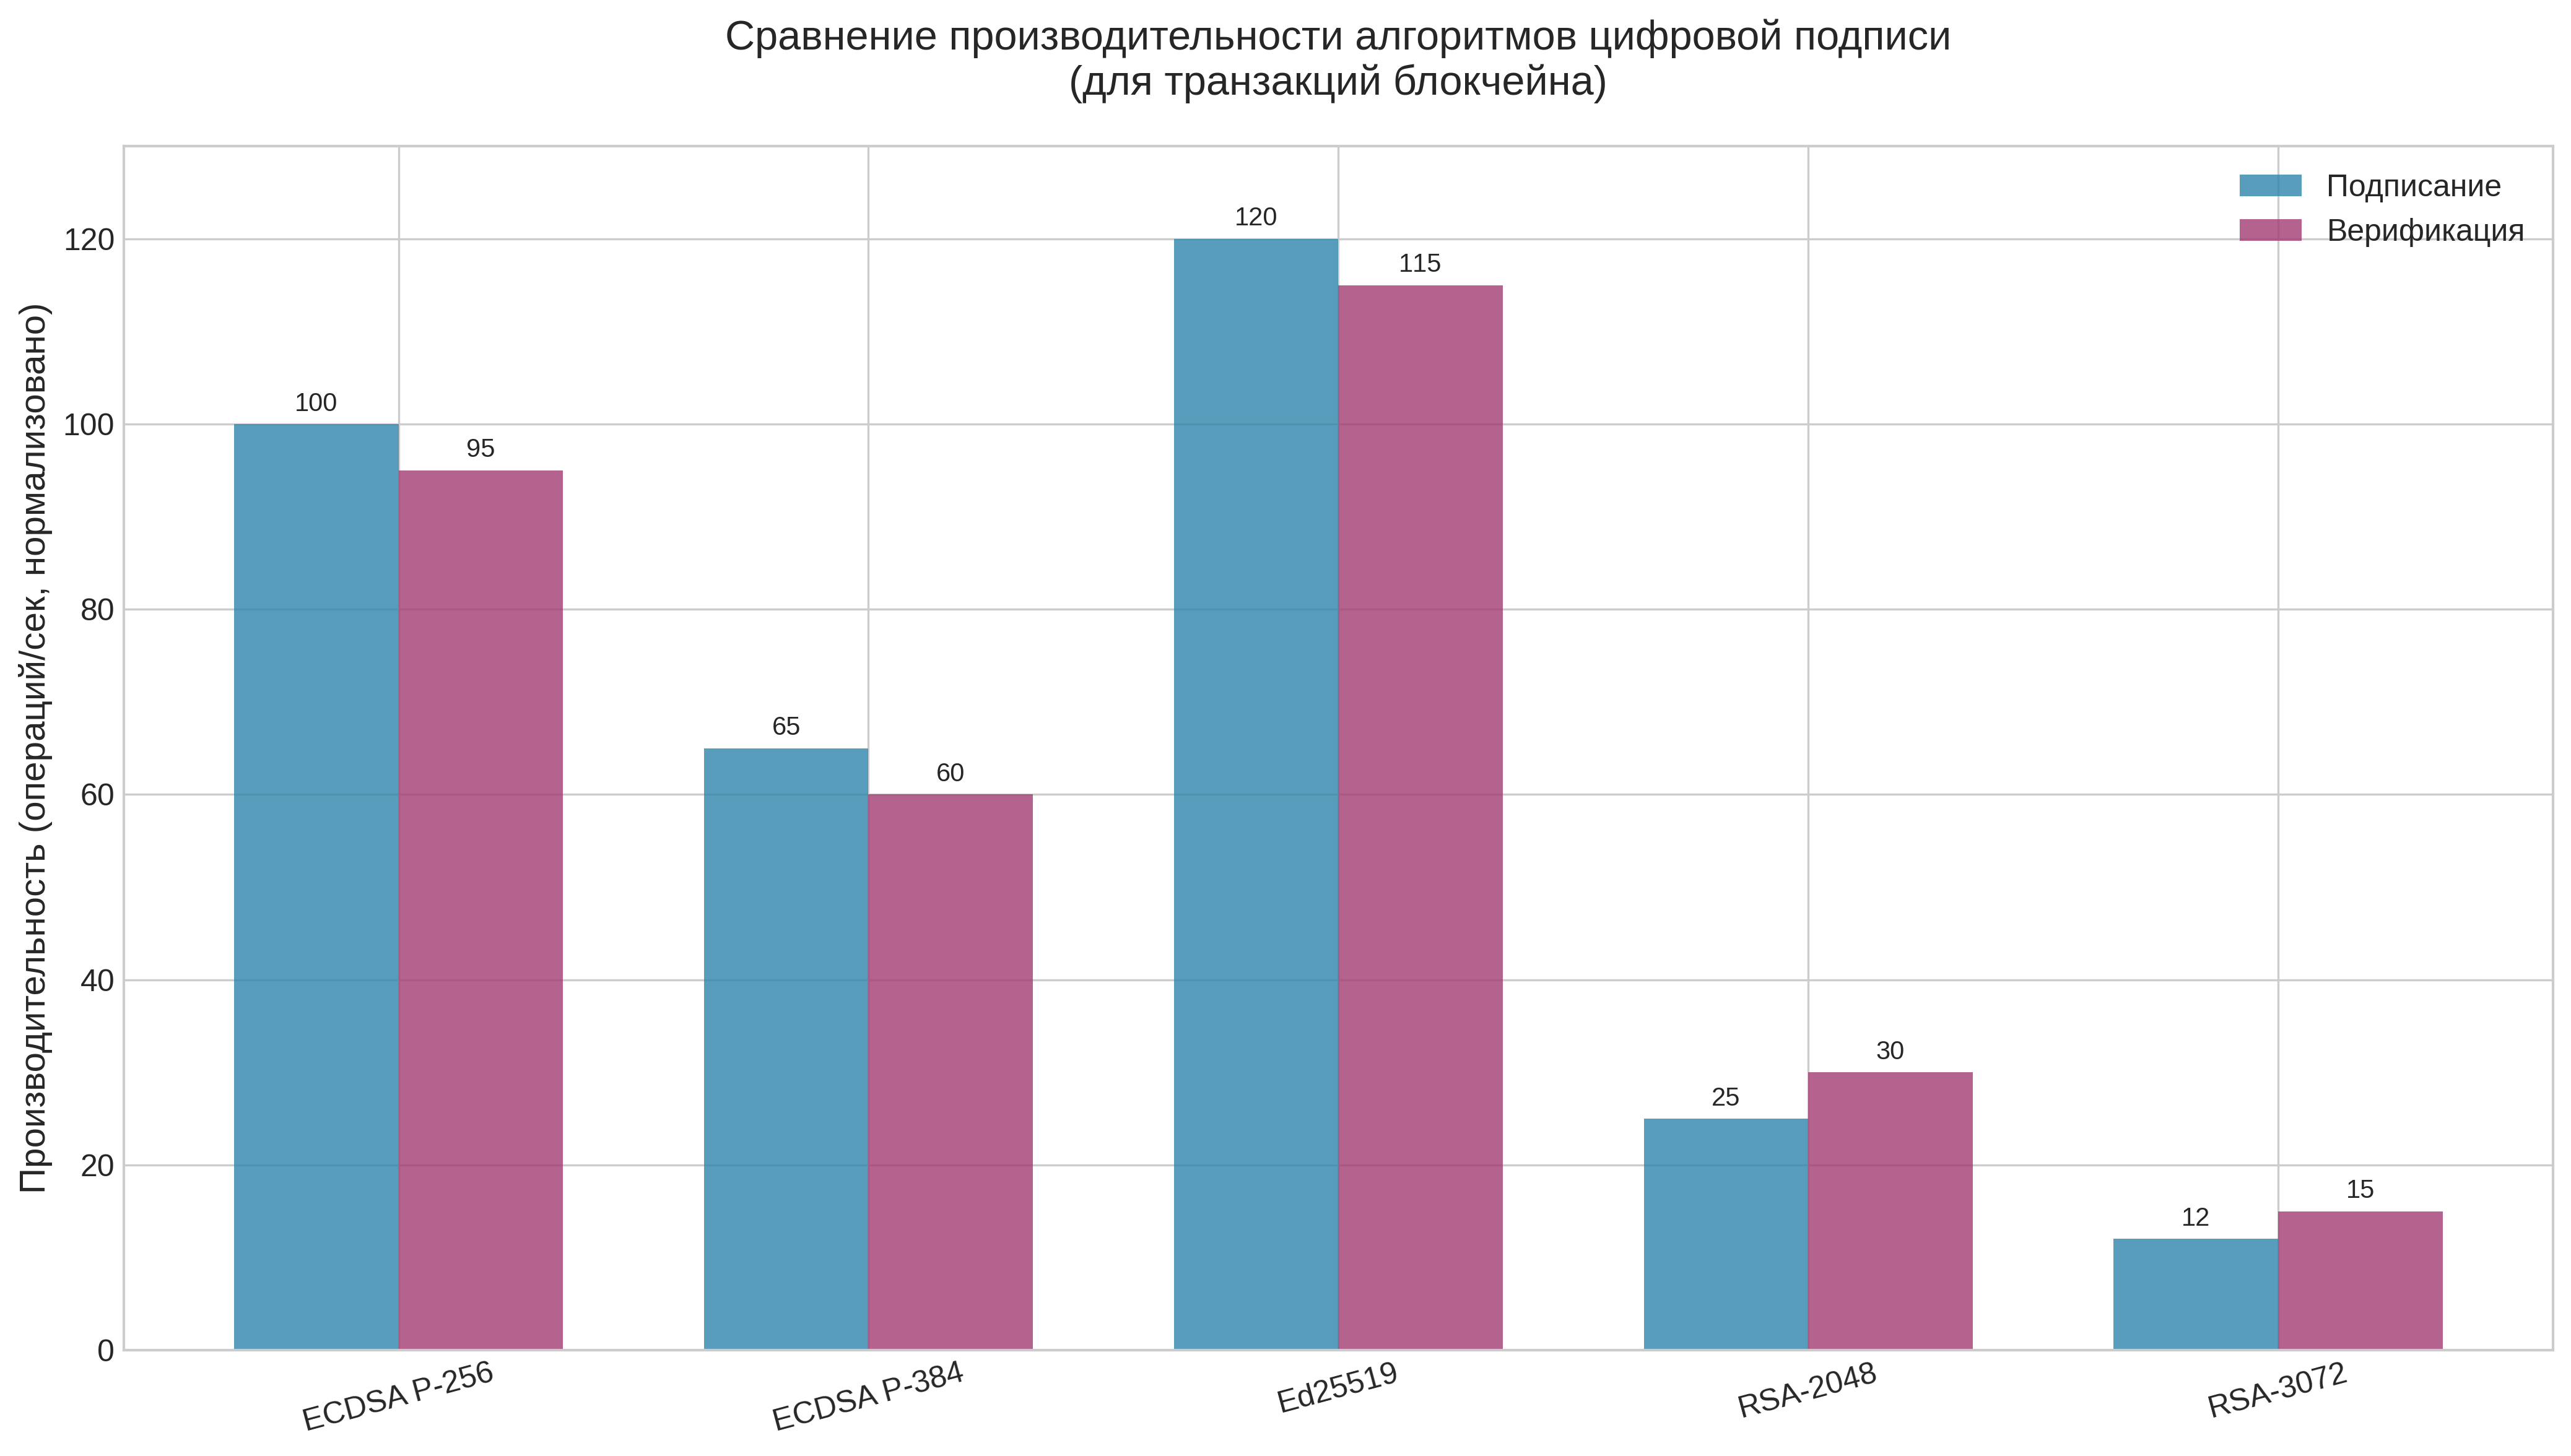
\includegraphics[width=0.9\textwidth]{crypto_charts/signature_performance.png}
    \caption{Сравнение производительности алгоритмов цифровой подписи}
    \label{fig:signature_perf}
    \source{Составлено автором}
\end{figure}

\textbf{Выводы:}
\begin{itemize}
    \item \textbf{Ed25519} показывает наилучшую производительность, но не поддерживается в Fabric;
    \item \textbf{ECDSA P-256} обеспечивает оптимальный баланс между скоростью и безопасностью;
    \item \textbf{RSA-2048/3072} значительно медленнее, что критично для высоконагруженных систем.
\end{itemize}

\section{Стойкость криптографических алгоритмов}

\begin{figure}[H]
    \centering
    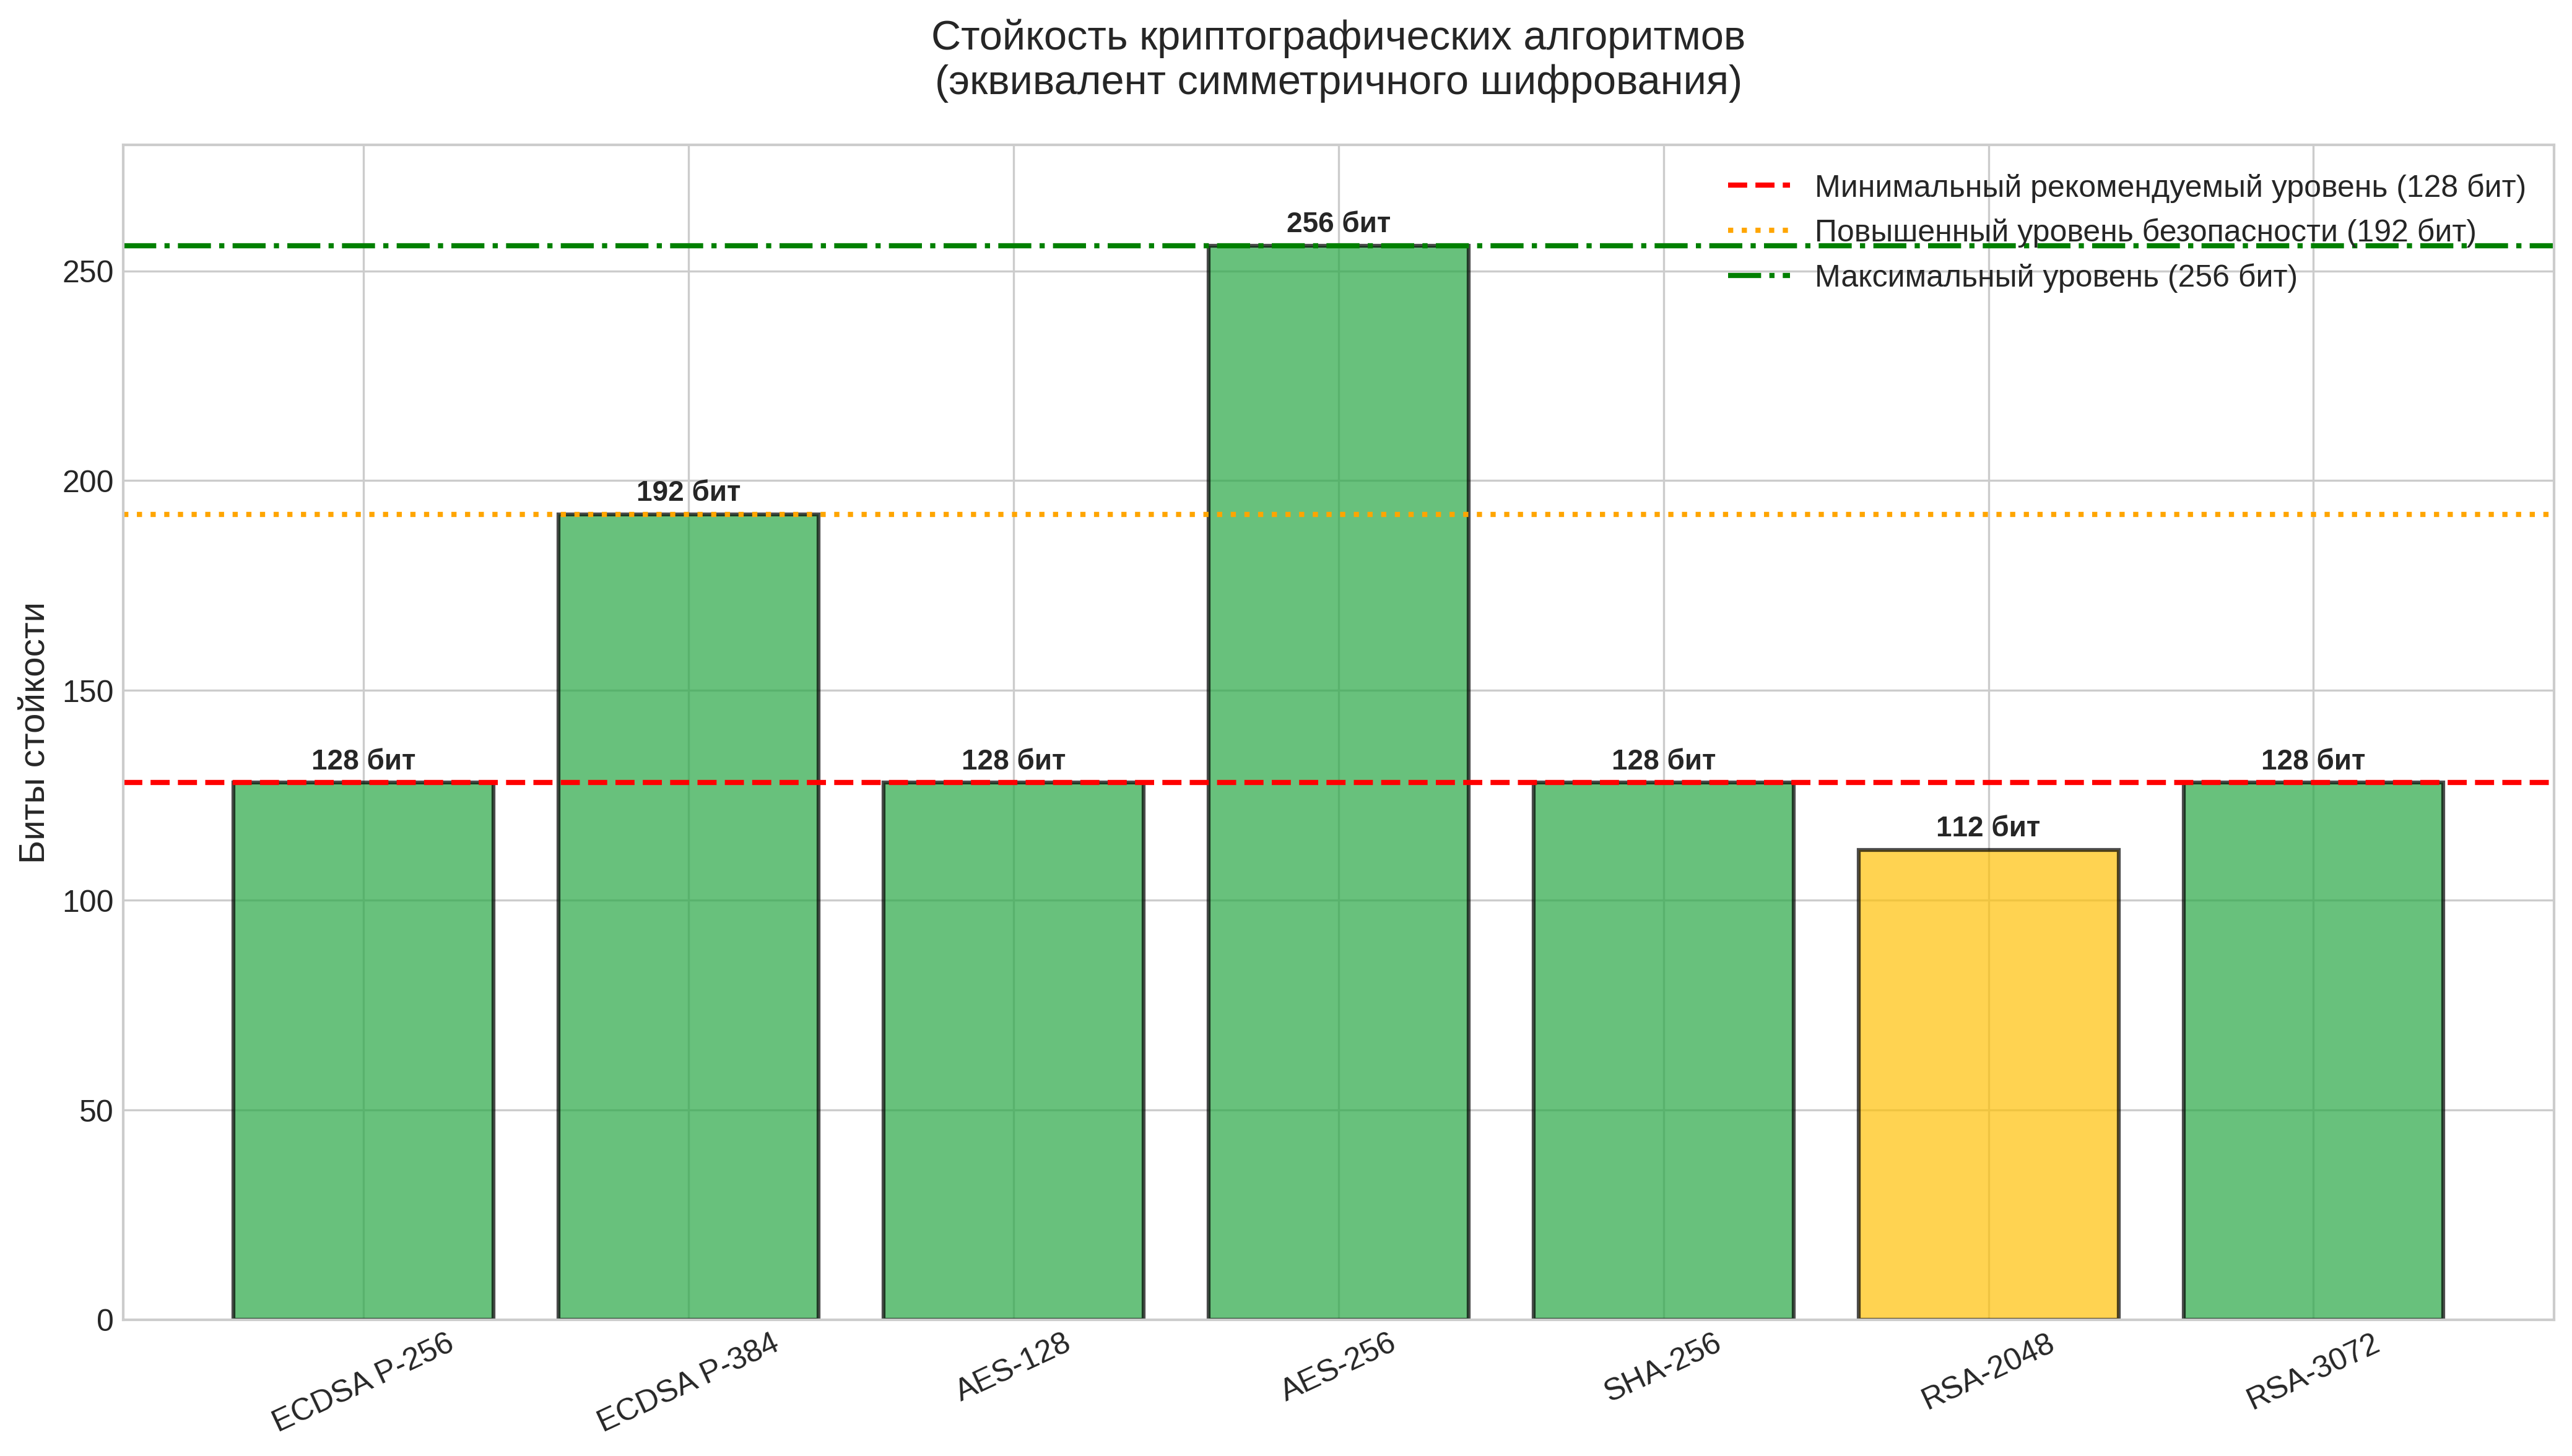
\includegraphics[width=0.9\textwidth]{crypto_charts/security_levels.png}
    \caption{Стойкость криптографических алгоритмов в битах}
    \label{fig:security_levels}
    \source{Составлено автором}
\end{figure}

\textbf{Выводы:}
\begin{itemize}
    \item Алгоритмы с уровнем стойкости $\ge$128 бит соответствуют современным требованиям NIST;
    \item \textbf{RSA-2048} (112 бит) требует замены на RSA-3072 или ECDSA;
    \item \textbf{AES-256} и \textbf{ECDSA P-384} обеспечивают повышенный уровень безопасности.
\end{itemize}

\section{Анализ реализации методов защиты}

\begin{figure}[H]
    \centering
    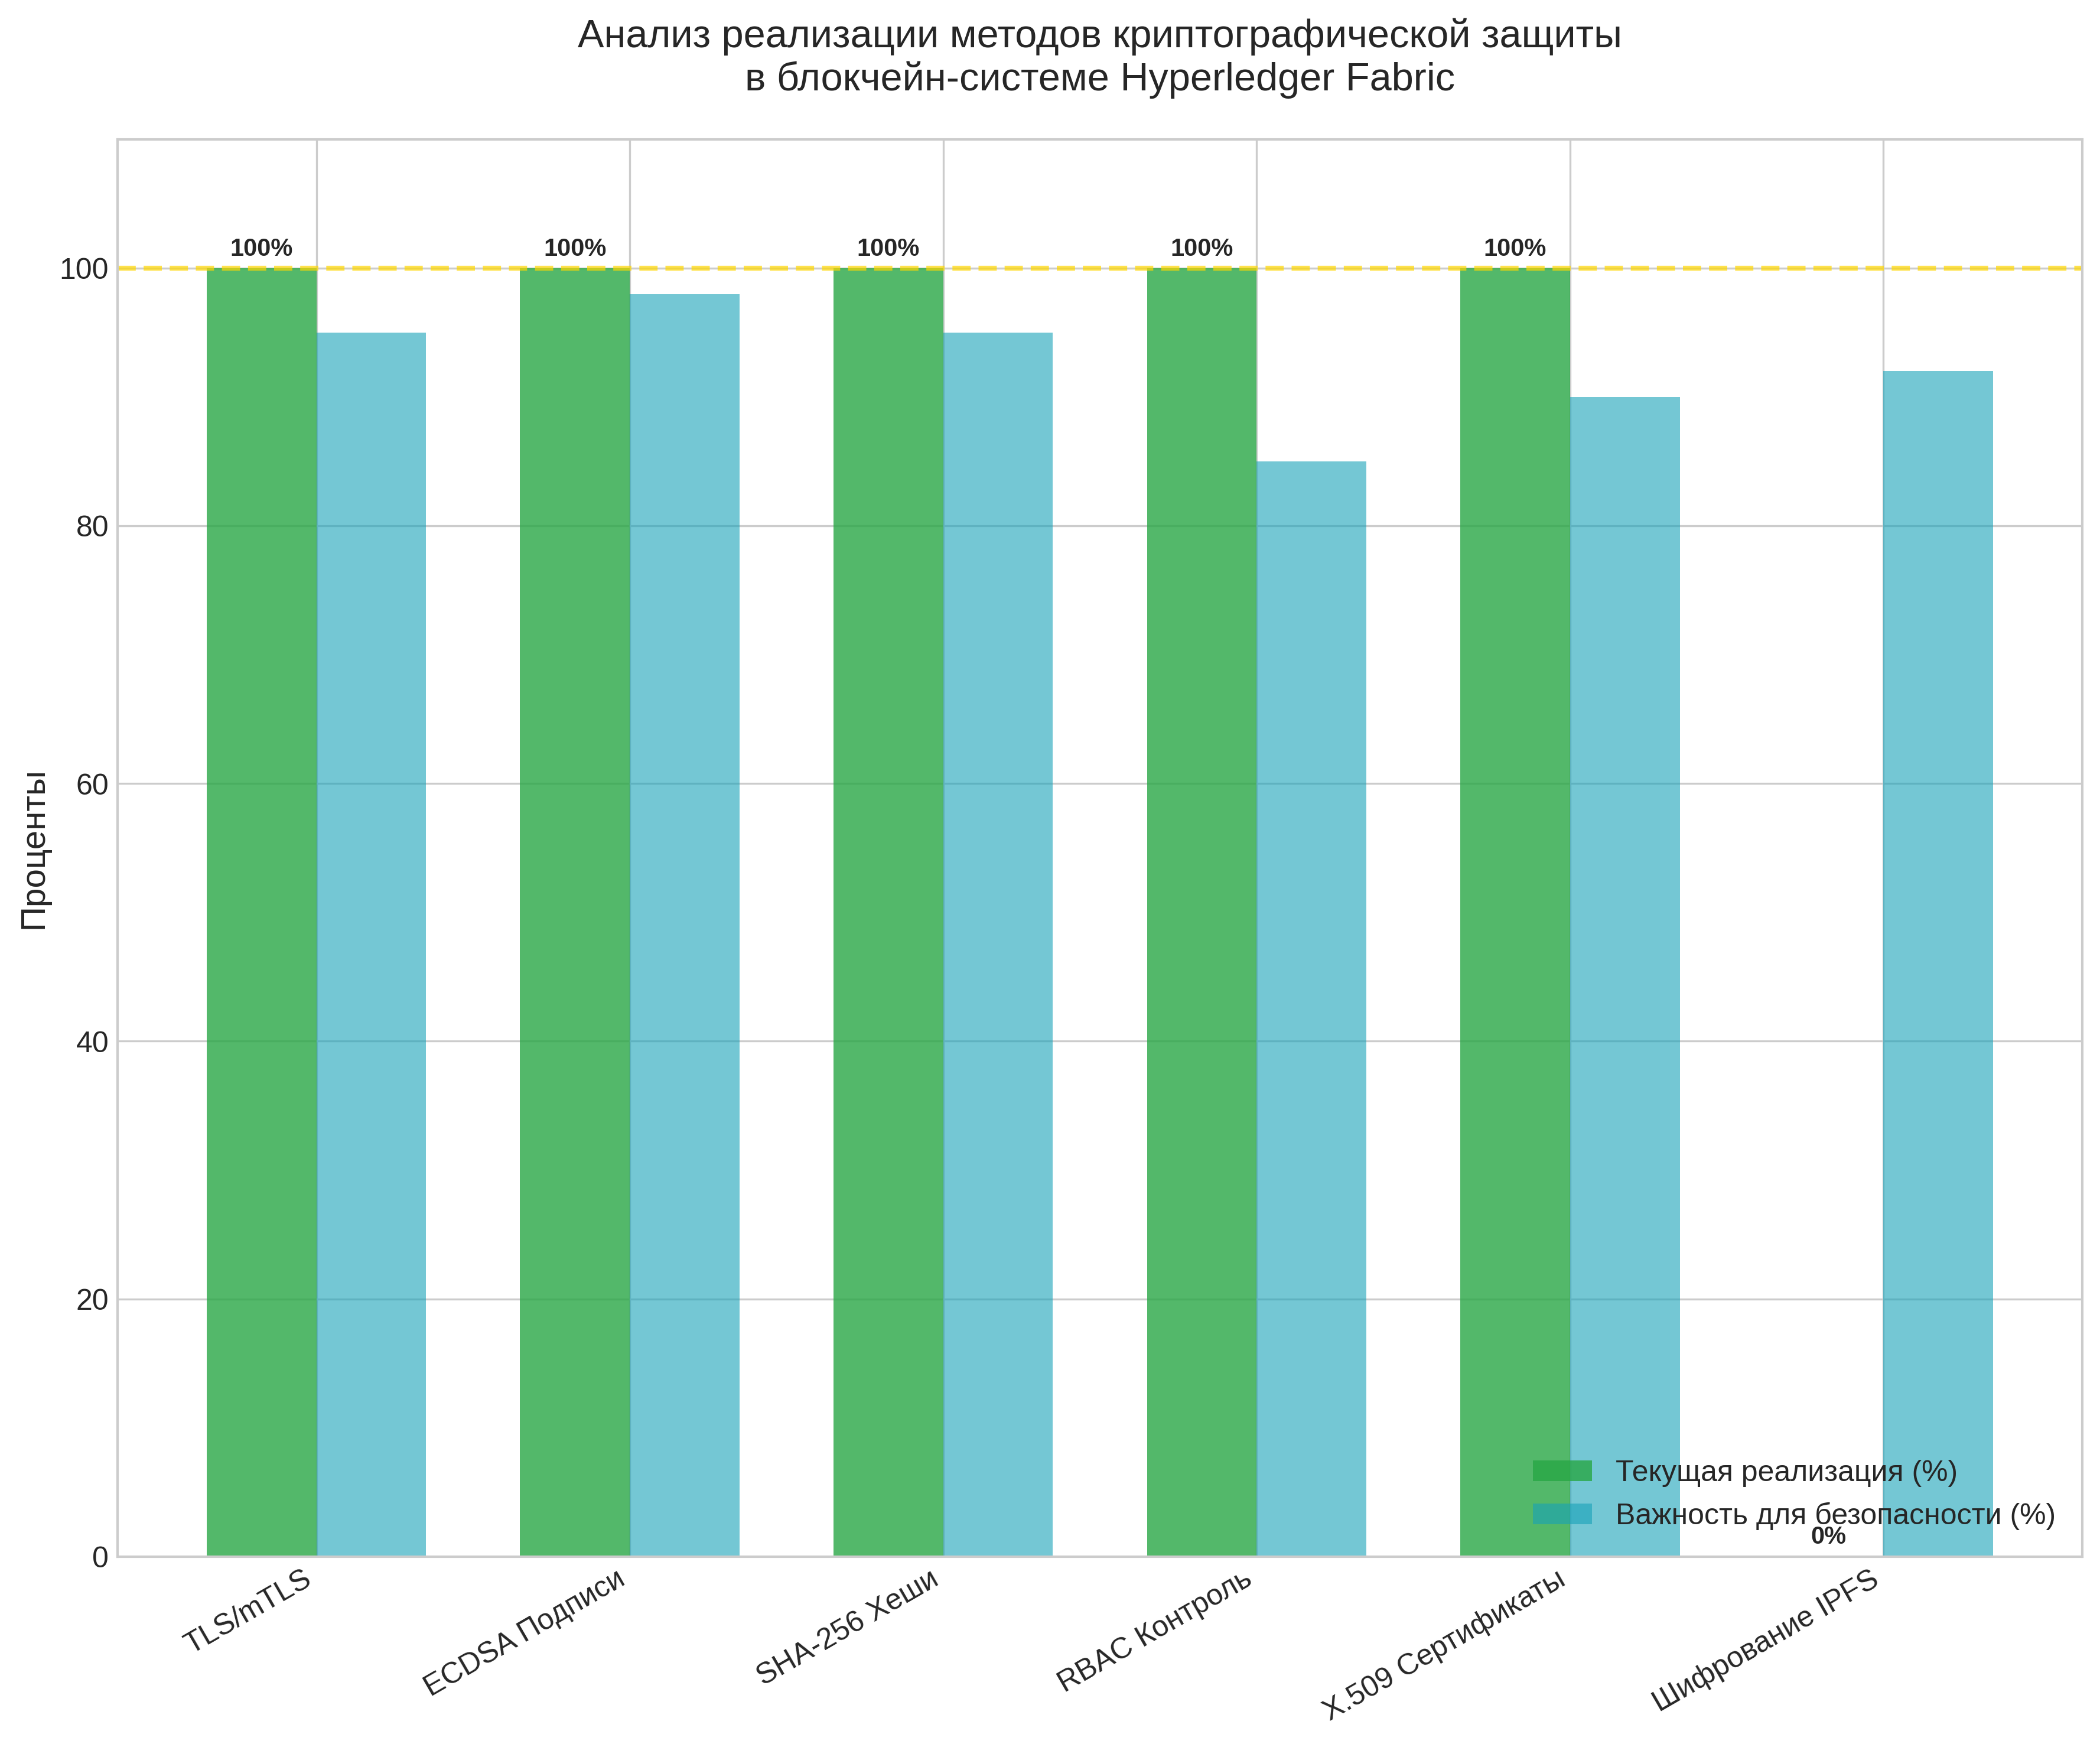
\includegraphics[width=0.9\textwidth]{crypto_charts/protection_analysis.png}
    \caption{Анализ реализации методов криптографической защиты}
    \label{fig:protection_analysis}
    \source{Составлено автором}
\end{figure}

\textbf{Выводы:}
\begin{itemize}
    \item Все базовые методы (TLS, ECDSA, SHA-256, RBAC, X.509) реализованы на 100\%;
    \item \textbf{Шифрование IPFS} не реализовано (0\%) при высокой важности (92\%);
    \item Требуется приоритетная реализация шифрования документов перед загрузкой в IPFS.
\end{itemize}

\section{Эволюция размеров ключей}

\begin{figure}[H]
    \centering
    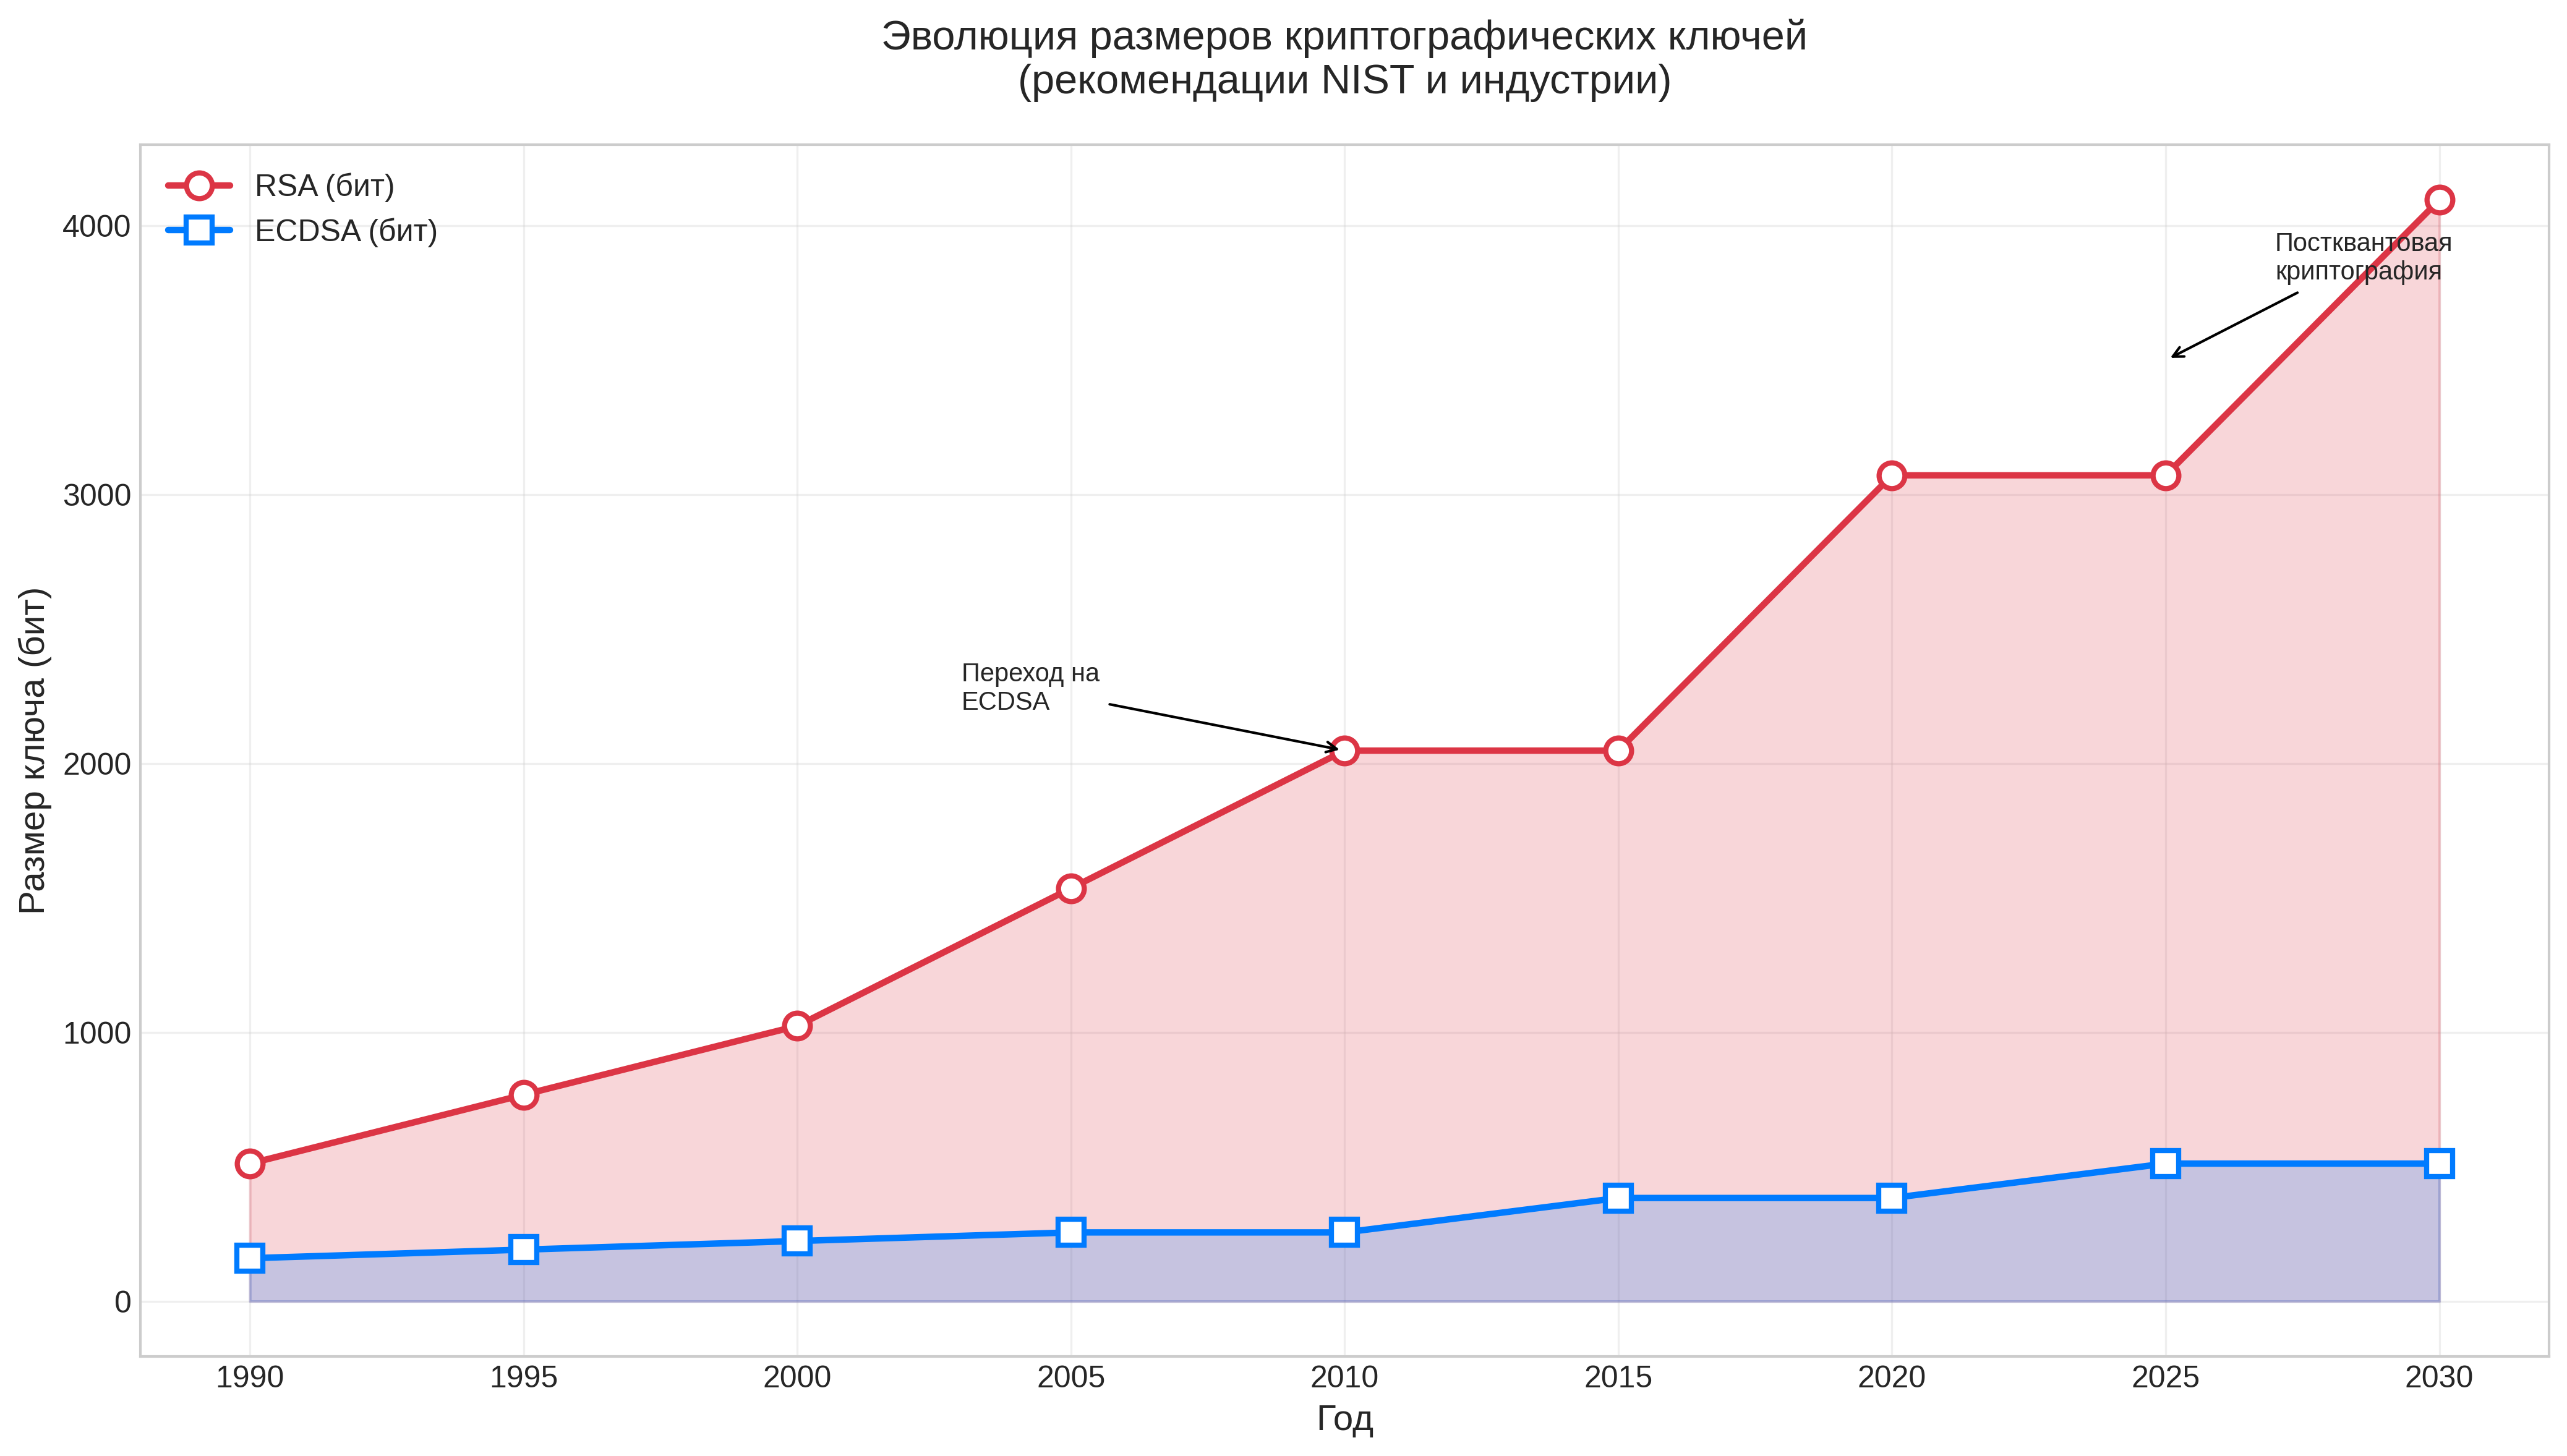
\includegraphics[width=0.9\textwidth]{crypto_charts/key_evolution.png}
    \caption{Эволюция размеров криптографических ключей (1990--2030 гг.)}
    \label{fig:key_evolution}
    \source{Составлено автором на основе рекомендаций NIST}
\end{figure}

\textbf{Выводы:}
\begin{itemize}
    \item Наблюдается постоянный рост требуемых размеров ключей;
    \item К 2025--2030 гг. ожидается переход на постквантовые алгоритмы;
    \item ECDSA требует значительно меньших размеров ключей при эквивалентной стойкости.
\end{itemize}

\section{Время выполнения операций}

\begin{figure}[H]
    \centering
    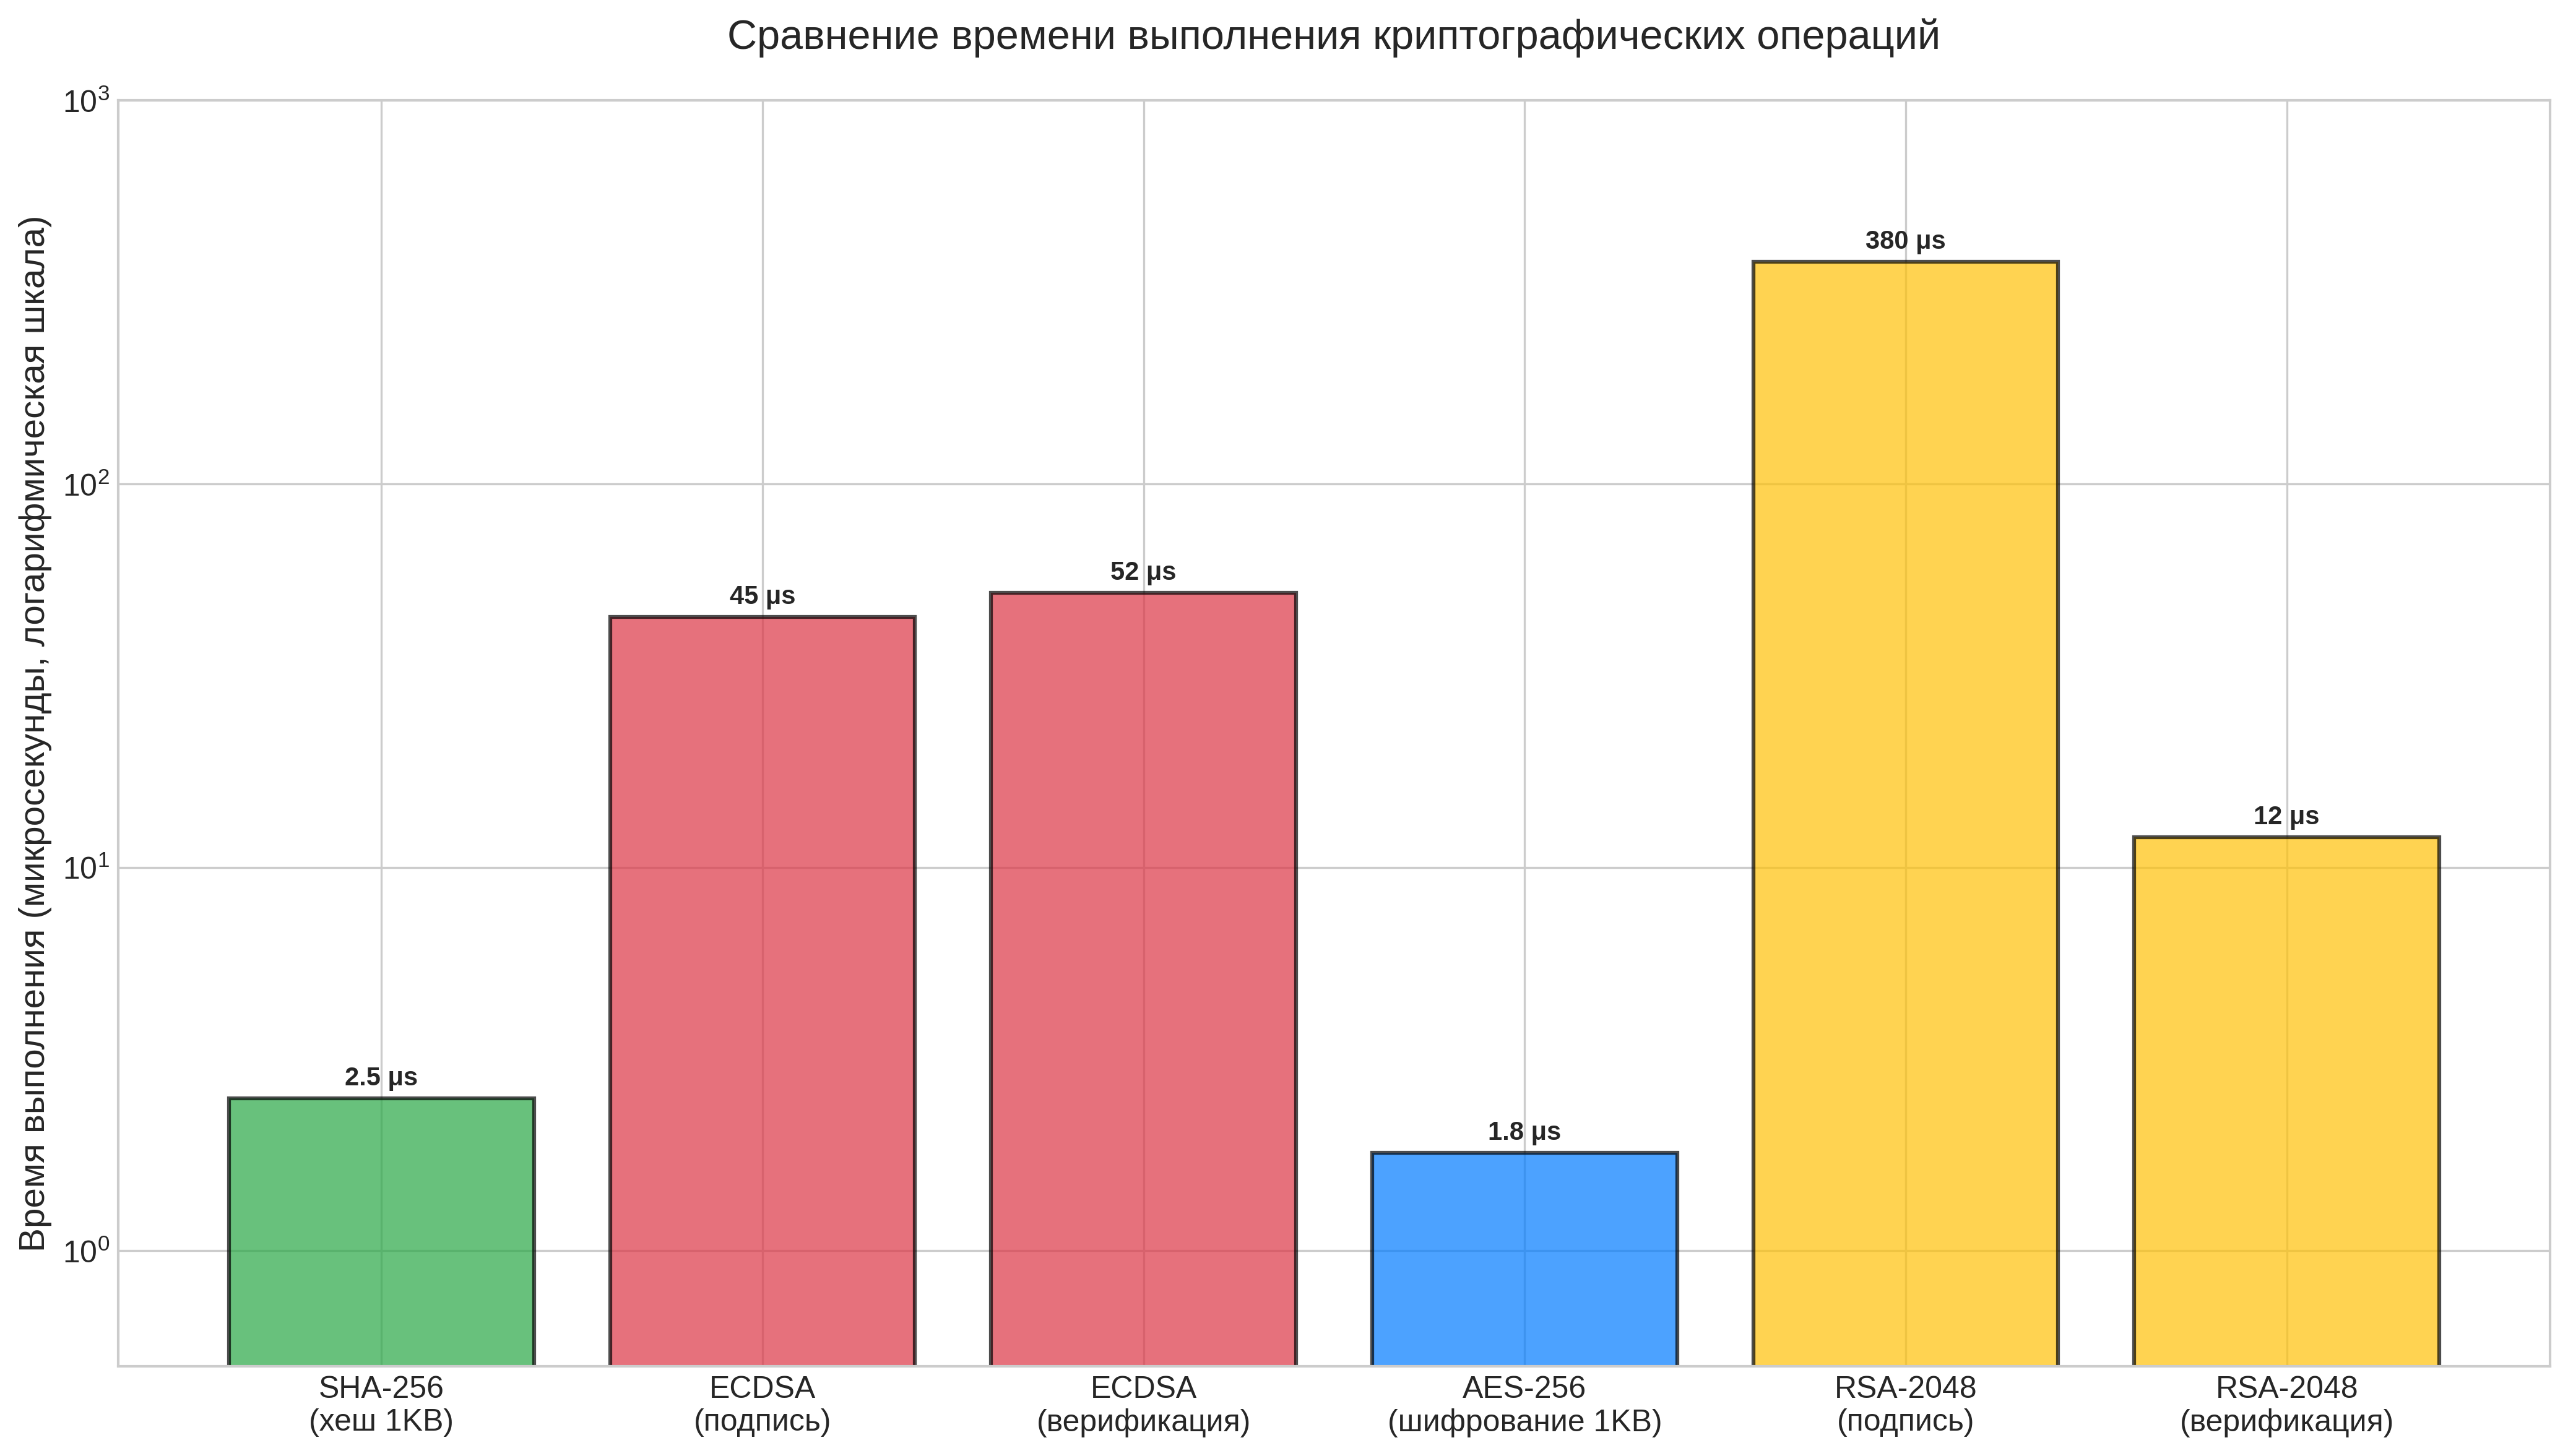
\includegraphics[width=0.9\textwidth]{crypto_charts/operation_time.png}
    \caption{Сравнение времени выполнения криптографических операций}
    \label{fig:operation_time}
    \source{Составлено автором}
\end{figure}

\textbf{Выводы:}
\begin{itemize}
    \item \textbf{SHA-256} и \textbf{AES-256} --- наиболее быстрые операции (1--3 мкс);
    \item \textbf{RSA-2048 подпись} --- самая медленная операция (380 мкс), в 76 раз медленнее ECDSA;
    \item Для блокчейн-систем предпочтительны ECDSA и симметричные алгоритмы.
\end{itemize}

\section{Матрица угроз безопасности}

\begin{figure}[H]
    \centering
    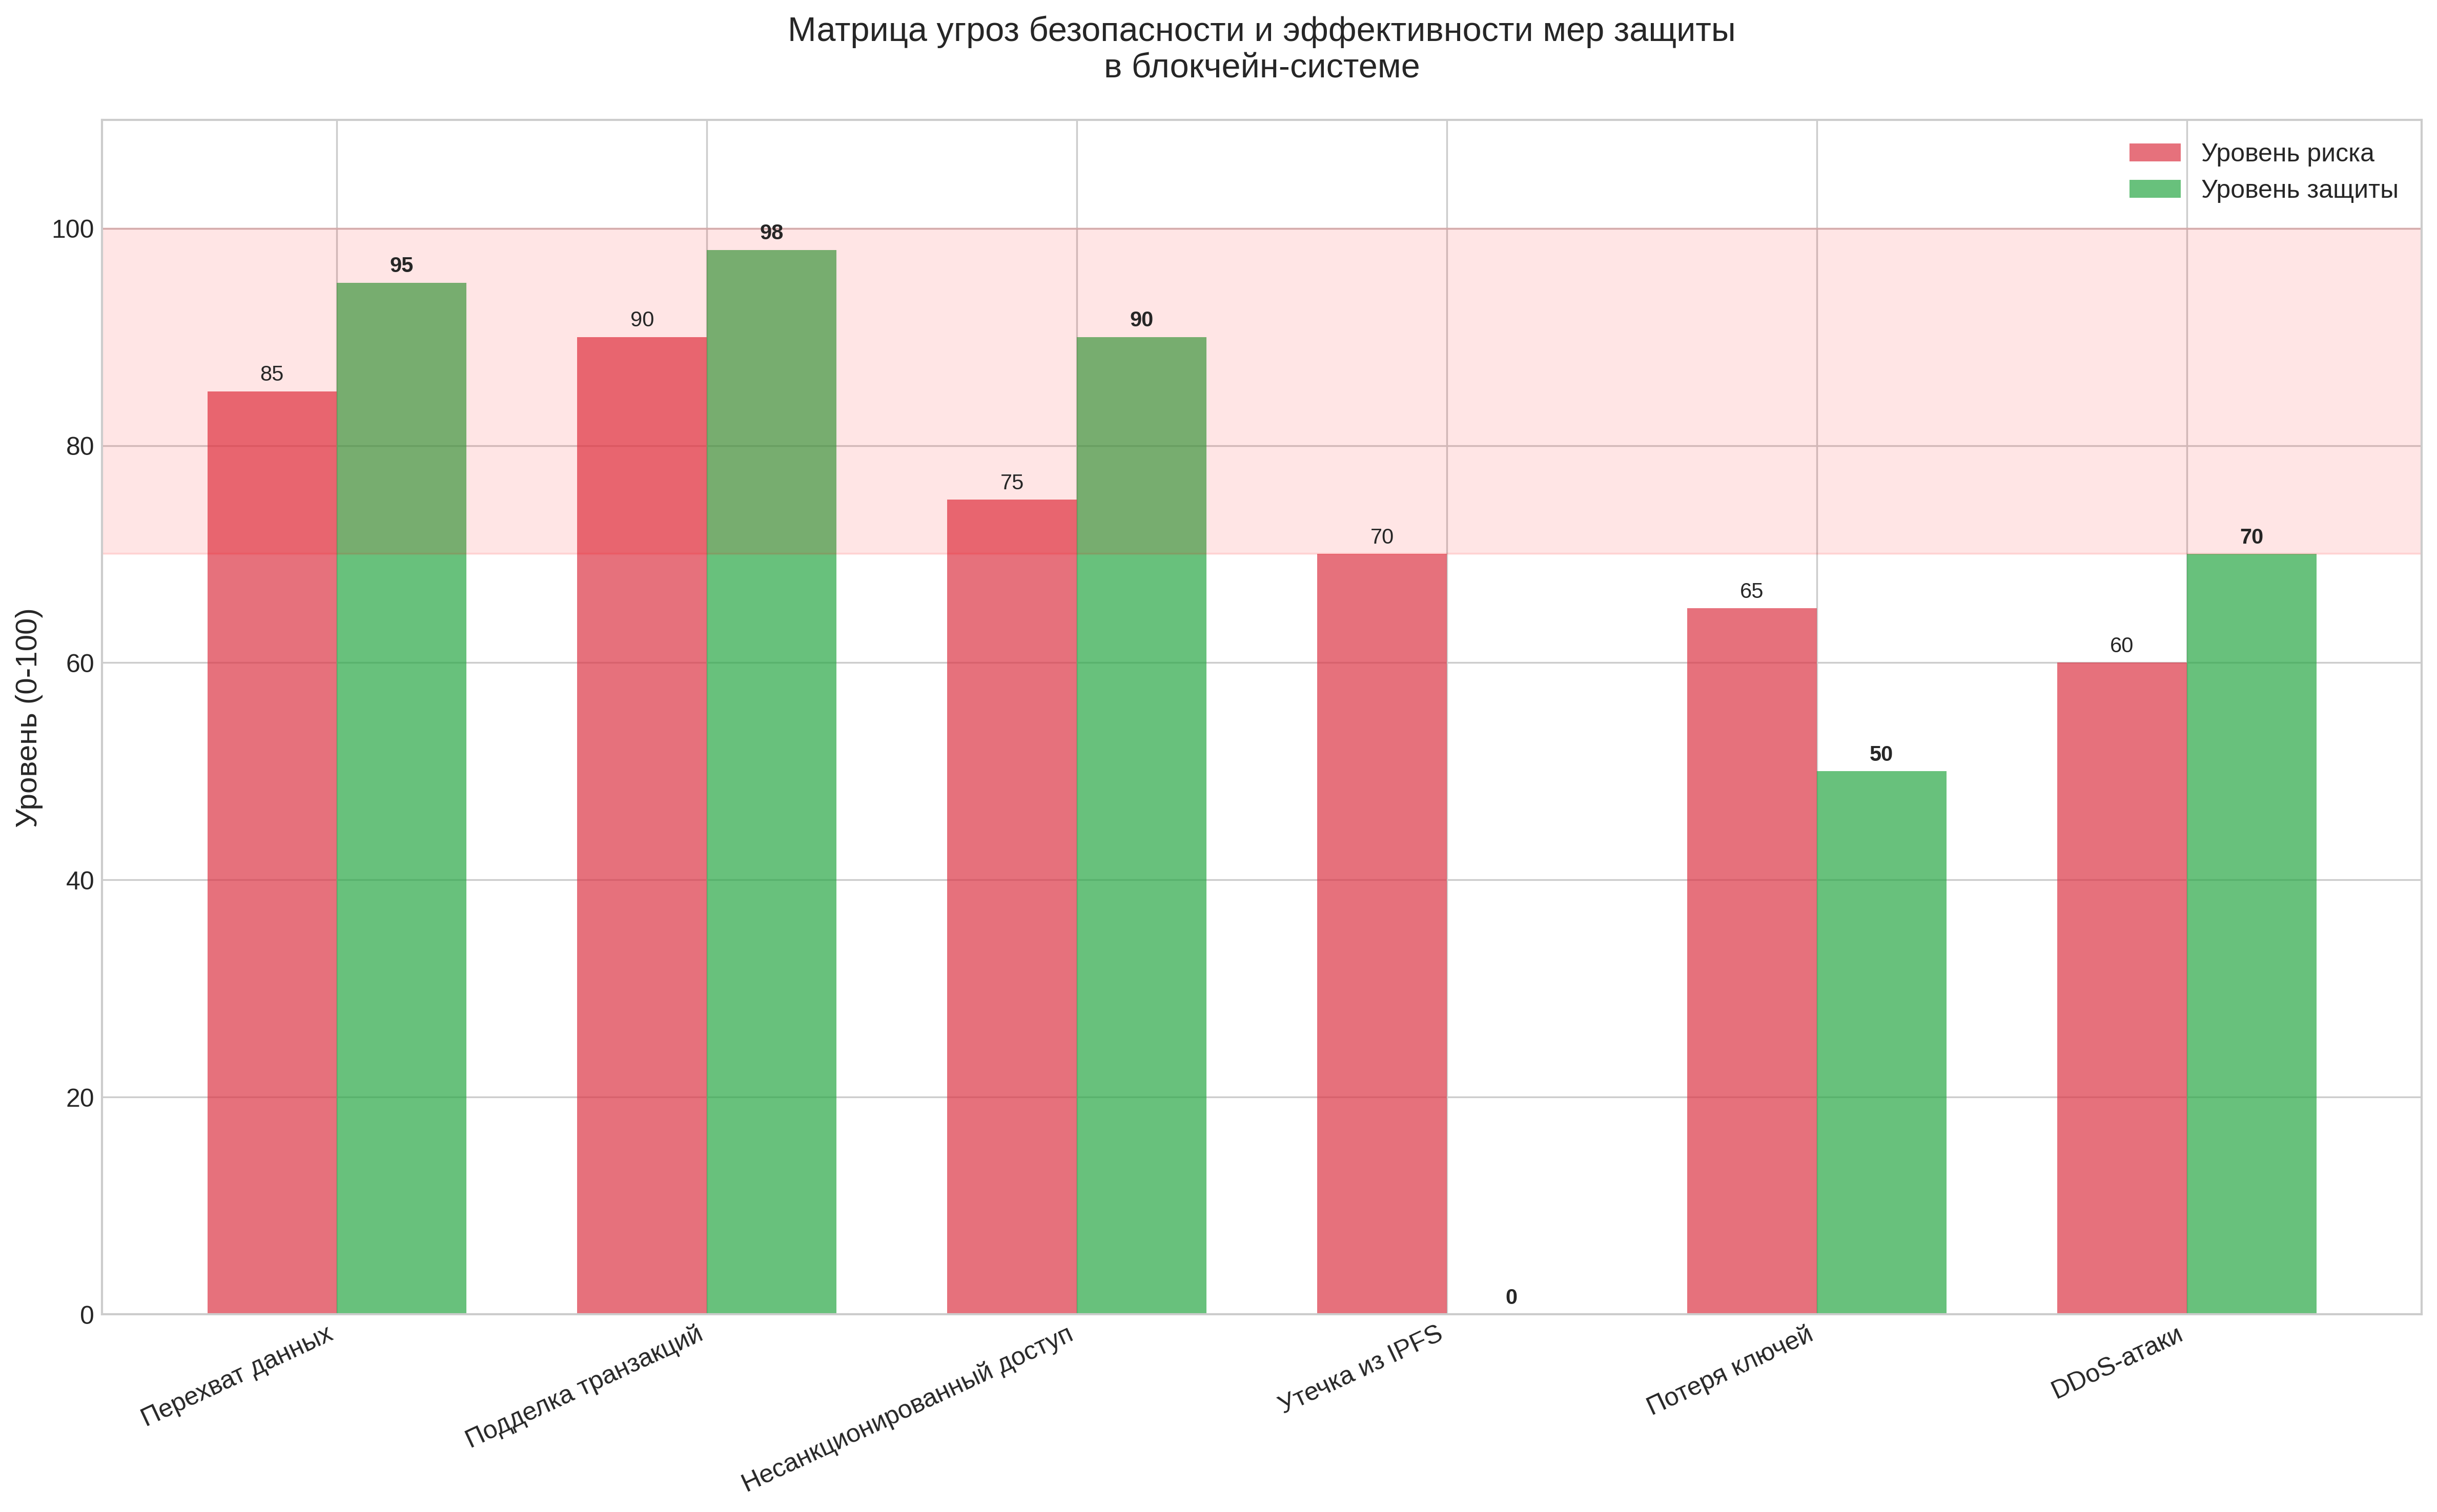
\includegraphics[width=0.9\textwidth]{crypto_charts/threat_matrix.png}
    \caption{Матрица угроз безопасности и эффективности мер защиты}
    \label{fig:threat_matrix}
    \source{Составлено автором}
\end{figure}

\textbf{Выводы:}
\begin{itemize}
    \item \textbf{Утечка из IPFS} --- критическая уязвимость (риск 70\%, защита 0\%);
    \item \textbf{Потеря ключей} --- средняя защита (50\%), требуется улучшение;
    \item Реализованные меры эффективно противодействуют основным угрозам.
\end{itemize}

\section{Постквантовая криптография}

\begin{figure}[H]
    \centering
    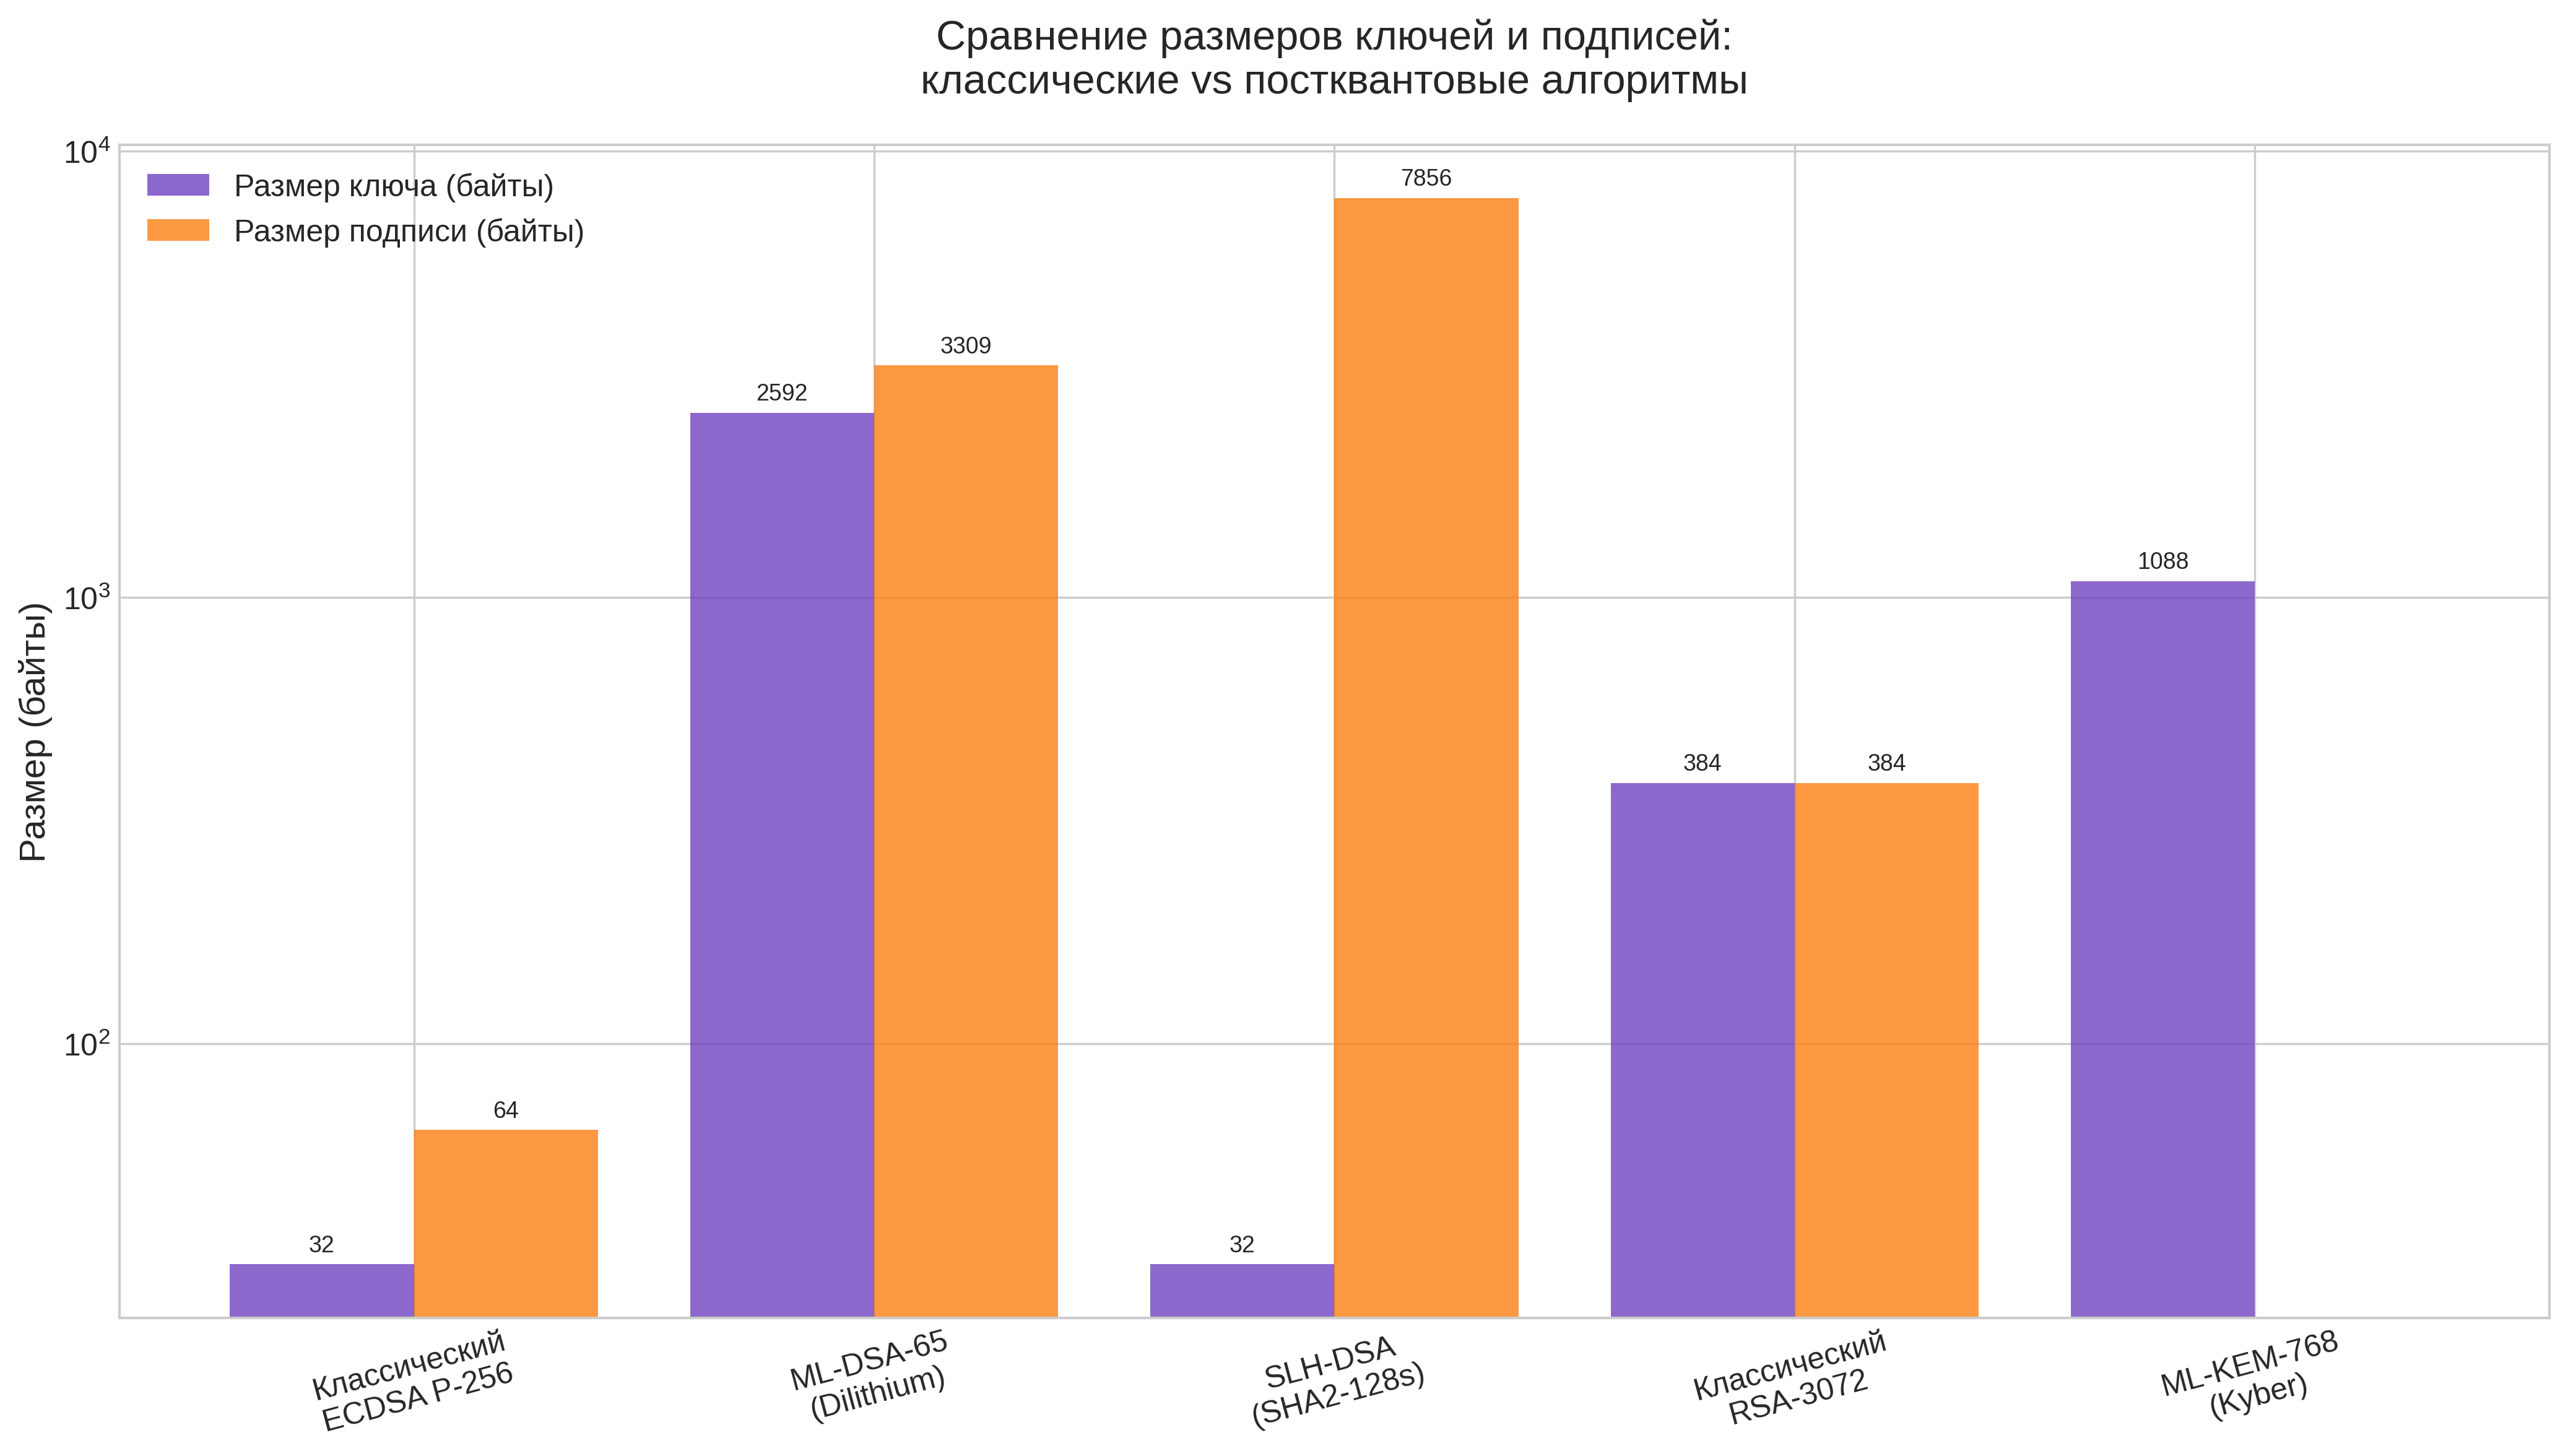
\includegraphics[width=0.9\textwidth]{crypto_charts/pqc_comparison.png}
    \caption{Сравнение классических и постквантовых алгоритмов}
    \label{fig:pqc_comparison}
    \source{Составлено автором на основе данных NIST}
\end{figure}

\textbf{Выводы:}
\begin{itemize}
    \item Постквантовые алгоритмы требуют значительно больших размеров ключей и подписей;
    \item \textbf{ML-DSA-65 (Dilithium)} --- рекомендуемый алгоритм для подписей (2592 байта ключ, 3309 байт подпись);
    \item Необходима подготовка инфраструктуры к увеличению размера данных в 50--100 раз.
\end{itemize}

\section{Архитектура системы защиты}

Архитектура многоуровневой системы криптографической защиты представлена на рисунке~\ref{fig:architecture}.

\begin{figure}[H]
    \centering
    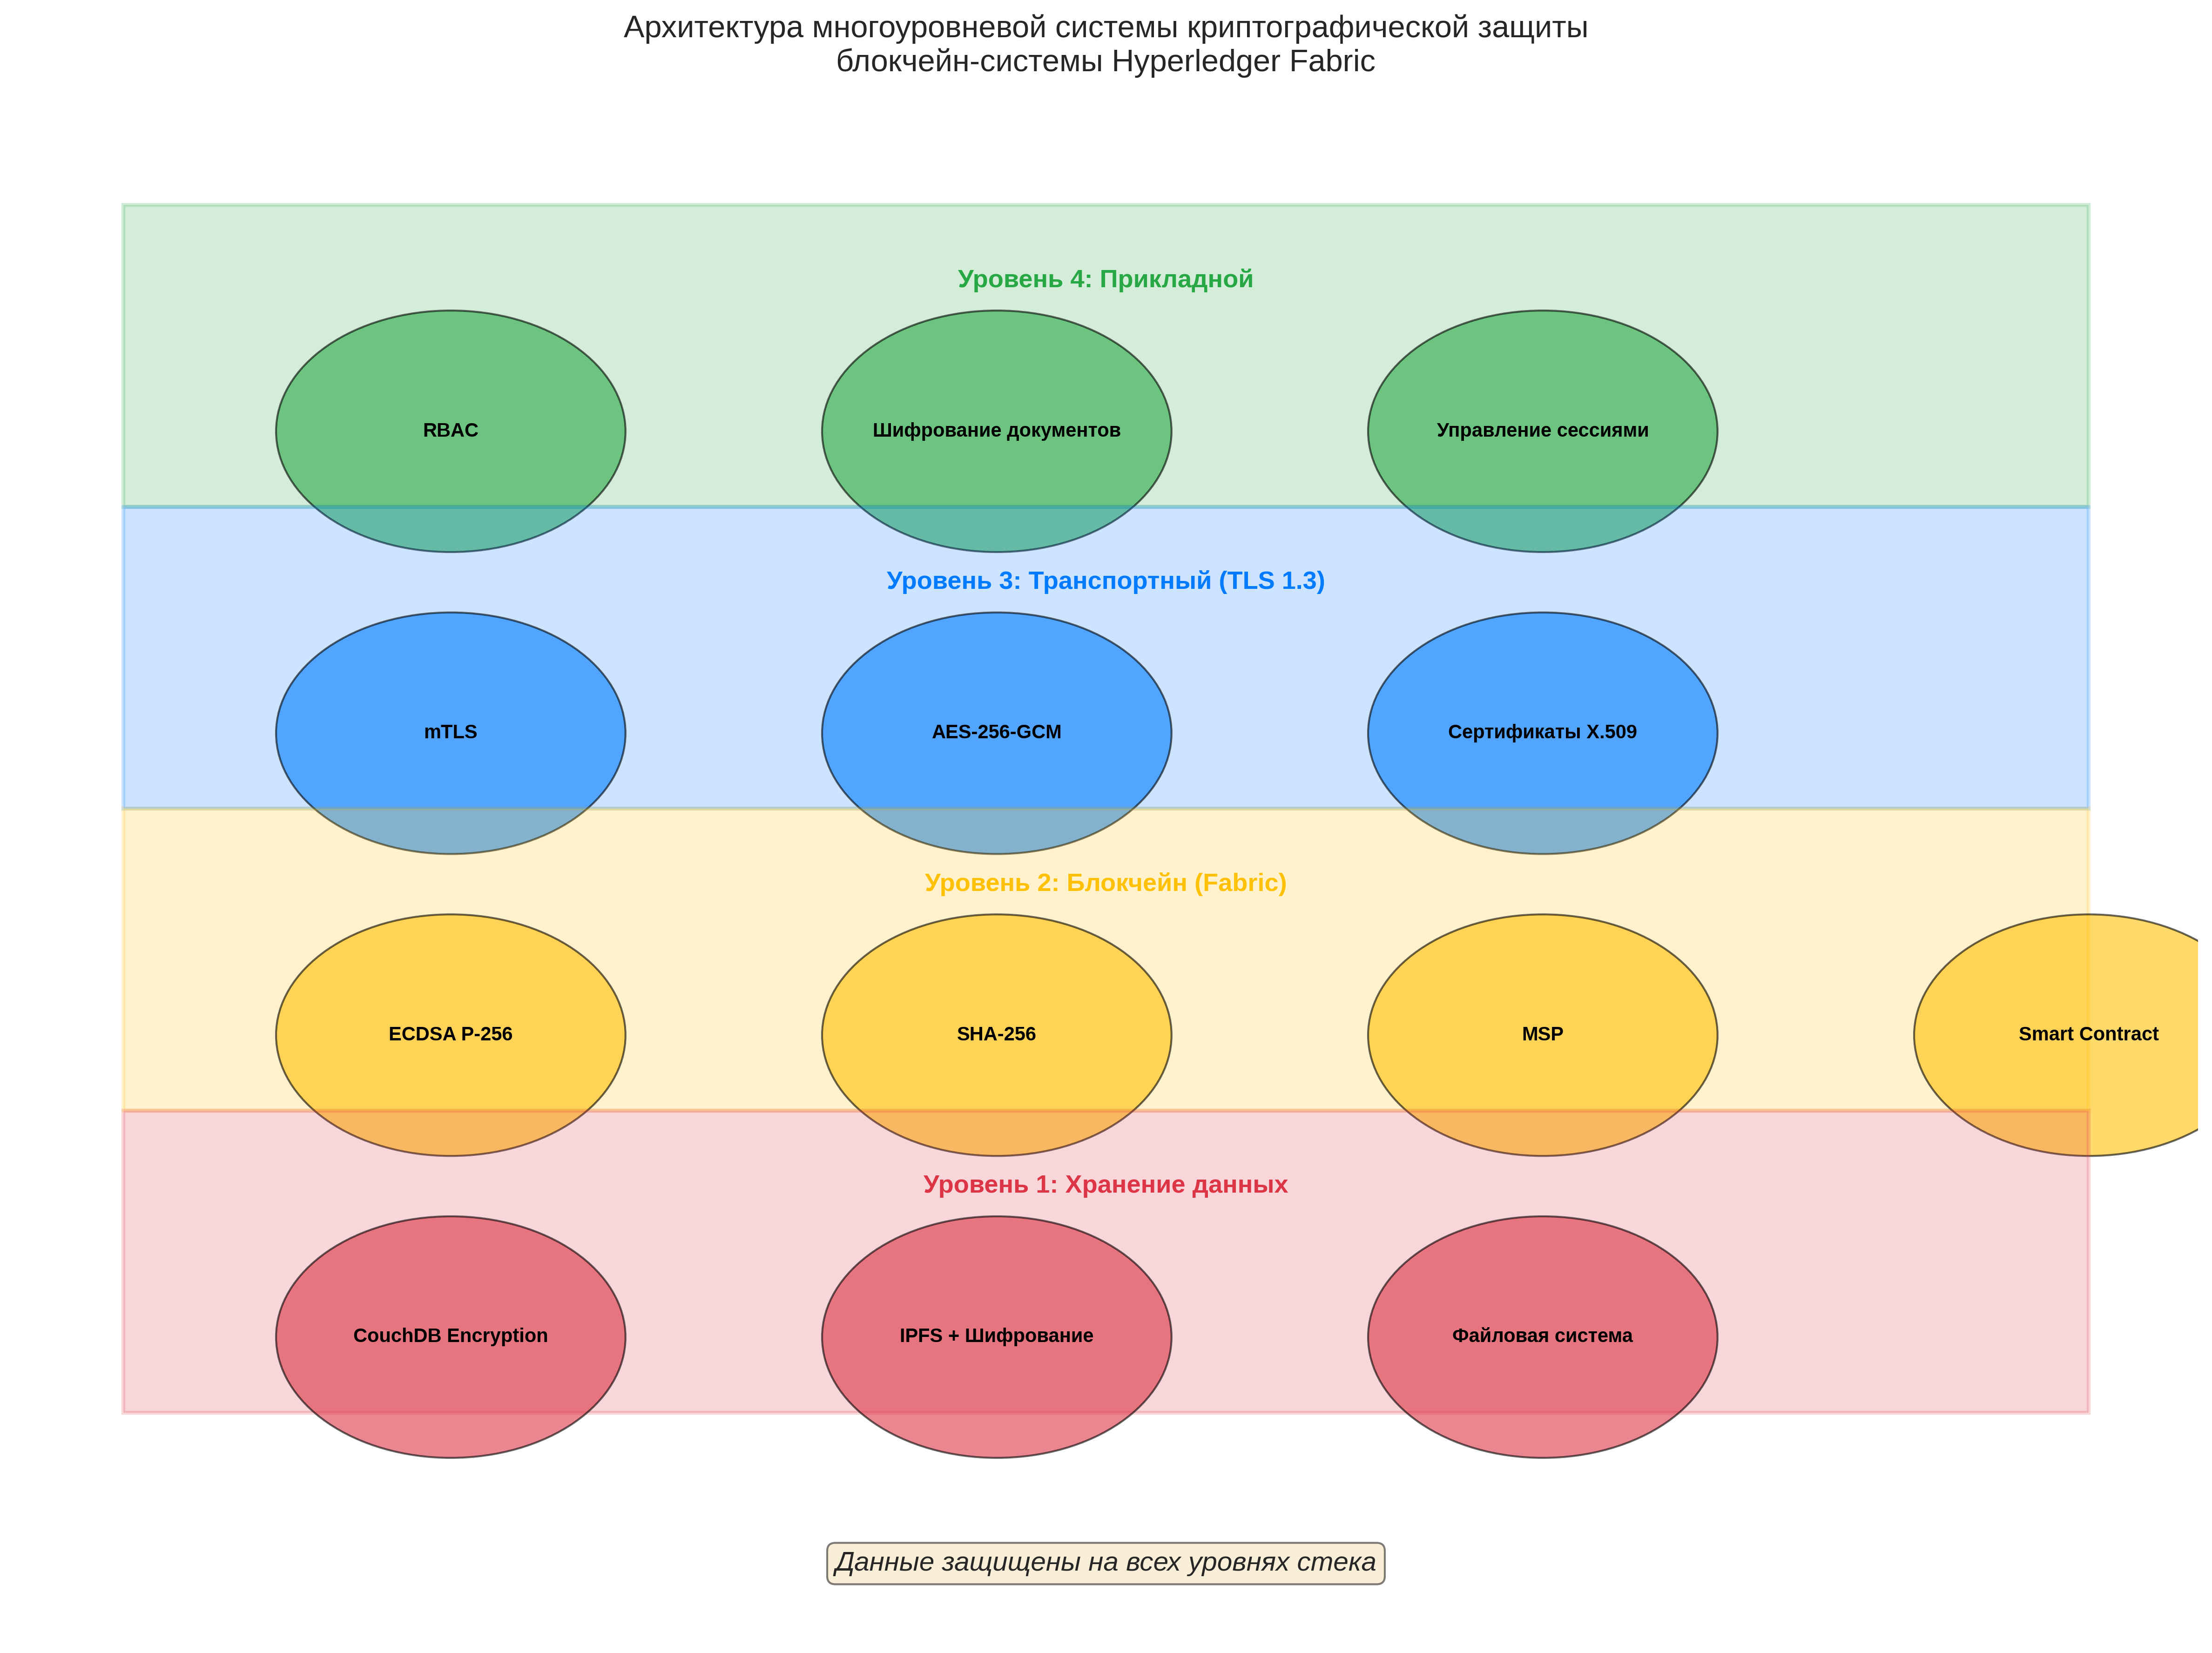
\includegraphics[width=0.9\textwidth]{crypto_charts/architecture_diagram.png}
    \caption{Архитектура многоуровневой системы криптографической защиты}
    \label{fig:architecture}
    \source{Составлено автором}
\end{figure}

\textbf{Уровни защиты:}
\begin{enumerate}
    \item \textbf{Уровень 1: Хранение данных} --- CouchDB Encryption, IPFS + Шифрование, Файловая система;
    \item \textbf{Уровень 2: Блокчейн (Fabric)} --- ECDSA P-256, SHA-256, MSP, Smart Contract;
    \item \textbf{Уровень 3: Транспортный (TLS 1.3)} --- mTLS, AES-256-GCM, Сертификаты X.509;
    \item \textbf{Уровень 4: Прикладной} --- RBAC, Шифрование документов, Управление сессиями.
\end{enumerate}

\newpage

% Глава 7: Сравнительная характеристика
\chapter{Сравнительная характеристика алгоритмов}

\section{Алгоритмы цифровой подписи}

\begin{table}[H]
\centering
\caption{Сравнение алгоритмов цифровой подписи}
\label{tab:signature_algorithms}
\begin{tabular}{|l|c|c|c|c|c|}
\hline
\textbf{Алгоритм} & \textbf{Размер ключа} & \textbf{Размер подписи} & \textbf{Скорость} & \textbf{Стойкость} & \textbf{Применение в Fabric} \\
\hline
ECDSA P-256 & 256 бит & 512 бит & Высокая & 128 бит & ✅ Основной \\
ECDSA P-384 & 384 бит & 768 бит & Средняя & 192 бит & ⚠️ Опционально \\
Ed25519 & 256 бит & 512 бит & Очень высокая & 128 бит & ❌ Не поддерживается \\
RSA-2048 & 2048 бит & 2048 бит & Низкая & 112 бит & ⚠️ Только для сертификатов \\
RSA-3072 & 3072 бит & 3072 бит & Очень низкая & 128 бит & ❌ Не используется \\
\hline
\end{tabular}
\end{table}

\section{Алгоритмы хеширования}

\begin{table}[H]
\centering
\caption{Сравнение алгоритмов хеширования}
\label{tab:hash_algorithms}
\begin{tabular}{|l|c|c|c|l|}
\hline
\textbf{Алгоритм} & \textbf{Размер хеша} & \textbf{Стойкость к коллизиям} & \textbf{Производительность} & \textbf{Применение} \\
\hline
SHA-256 & 256 бит & $2^{128}$ & Высокая & ✅ Fabric, IPFS \\
SHA-384 & 384 бит & $2^{192}$ & Высокая & ⚠️ Опционально \\
SHA3-256 & 256 бит & $2^{128}$ & Средняя & ⚠️ IPFS CID v1 \\
BLAKE2b & 256 бит & $2^{128}$ & Очень высокая & ⚠️ IPFS CID v1 \\
MD5 & 128 бит & $<2^{20}$ & Очень высокая & ❌ Небезопасен \\
\hline
\end{tabular}
\end{table}

\section{Алгоритмы симметричного шифрования}

\begin{table}[H]
\centering
\caption{Сравнение алгоритмов симметричного шифрования}
\label{tab:symmetric_algorithms}
\begin{tabular}{|l|c|c|c|l|}
\hline
\textbf{Алгоритм} & \textbf{Размер ключа} & \textbf{Режим} & \textbf{Производительность} & \textbf{Применение} \\
\hline
AES-128 & 128 бит & GCM & Очень высокая & ✅ TLS \\
AES-256 & 256 бит & GCM & Высокая & ✅ TLS (рекомендуется) \\
ChaCha20 & 256 бит & Poly1305 & Очень высокая & ✅ TLS (альтернатива) \\
DES & 56 бит & CBC & Низкая & ❌ Небезопасен \\
3DES & 168 бит & CBC & Очень низкая & ❌ Устарел \\
\hline
\end{tabular}
\end{table}

\newpage

% Глава 8: Рекомендации
\chapter{Рекомендации по улучшению}

\section{Краткосрочные улучшения (1--3 месяца)}

\subsection{Внедрение шифрования документов перед загрузкой в IPFS}

Рекомендуется использовать AES-256-GCM для шифрования документов. Пример реализации:

\begin{lstlisting}[caption=Пример шифрования документов,captionpos=b]
from cryptography.hazmat.primitives.ciphers.aead import AESGCM
import os

class DocumentEncryptor:
    def __init__(self, key=None):
        if key is None:
            self.key = AESGCM.generate_key(bit_length=256)
        else:
            self.key = key
        self.aesgcm = AESGCM(self.key)
    
    def encrypt(self, plaintext, associated_data=b''):
        nonce = os.urandom(12)  # 96-bit nonce for GCM
        ciphertext = self.aesgcm.encrypt(nonce, plaintext, 
                                          associated_data)
        return nonce + ciphertext
\end{lstlisting}

\subsection{Усиление защиты приватных ключей}

\begin{itemize}
    \item Использование аппаратных модулей безопасности (HSM);
    \item Внедрение пороговой криптографии (threshold cryptography);
    \item Регулярная ротация ключей.
\end{itemize}

\subsection{Обновление параметров TLS}

\begin{lstlisting}[language=YAML,caption=Рекомендуемая конфигурация TLS,captionpos=b]
tls:
  min_version: TLSv1.3
  cipher_suites:
    - TLS_AES_256_GCM_SHA384
    - TLS_CHACHA20_POLY1305_SHA256
  curve_preference:
    - X25519
    - secp384r1
\end{lstlisting}

\section{Долгосрочные улучшения (6--12 месяцев)}

\subsection{Переход на постквантовую криптографию}

\begin{table}[H]
\centering
\caption{Рекомендуемые постквантовые алгоритмы (NIST 2024)}
\label{tab:pqc_algorithms}
\begin{tabular}{|l|l|c|c|}
\hline
\textbf{Категория} & \textbf{Алгоритм} & \textbf{Размер ключа} & \textbf{Размер подписи} \\
\hline
KEM & ML-KEM-768 (Kyber) & 1088 байт & -- \\
Signature & ML-DSA-65 (Dilithium) & 2592 байт & 3309 байт \\
Signature & SLH-DSA-SHA2-128s & 32 байт & 7856 байт \\
\hline
\end{tabular}
\end{table}

\subsection{Внедрение Zero-Knowledge Proofs}

Для повышения конфиденциальности транзакций:
\begin{itemize}
    \item \textbf{zk-SNARKs} --- для верификации без раскрытия данных;
    \item \textbf{zk-STARKs} --- для масштабируемых доказательств.
\end{itemize}

\subsection{Конфиденциальные вычисления (Confidential Computing)}

\begin{itemize}
    \item Использование Intel SGX или AMD SEV;
    \item Защищённые анклавы для выполнения chaincode;
    \item Шифрование данных в процессе обработки.
\end{itemize}

\section{Организационные меры}

\subsection{Политика управления ключами}

\begin{itemize}
    \item Пользовательские ключи: каждые 90 дней;
    \item Ключи узлов (peers): каждые 180 дней;
    \item Корневые сертификаты CA: каждые 365 дней;
    \item Ключи шифрования данных: при каждом изменении состава участников.
\end{itemize}

\subsection{Мониторинг и аудит}

\begin{itemize}
    \item Логирование всех криптографических операций;
    \item Мониторинг попыток несанкционированного доступа;
    \item Регулярный аудит безопасности.
\end{itemize}

\newpage

% Глава 9: Заключение
\chapter{Заключение}

\section{Основные выводы}

\begin{enumerate}
    \item \textbf{Текущее состояние криптографической защиты:}
    \begin{itemize}
        \item Hyperledger Fabric предоставляет надёжную базовую защиту с использованием ECDSA P-256 и SHA-256;
        \item TLS защищает каналы связи между компонентами системы;
        \item Система RBAC обеспечивает контроль доступа на уровне приложений.
    \end{itemize}
    
    \item \textbf{Выявленные области для улучшения:}
    \begin{itemize}
        \item Отсутствие шифрования документов в IPFS;
        \item Необходимость усиления защиты приватных ключей;
        \item Потребность в подготовке к постквантовой эре.
    \end{itemize}
    
    \item \textbf{Рекомендуемый план действий:}
    \begin{itemize}
        \item Краткосрочно: внедрить шифрование документов перед загрузкой в IPFS;
        \item Среднесрочно: обновить параметры TLS и внедрить HSM;
        \item Долгосрочно: подготовить миграцию на постквантовые алгоритмы.
    \end{itemize}
\end{enumerate}

\section{Научная новизна}

В рамках данного исследования:
\begin{itemize}
    \item Проведён комплексный анализ криптографических методов в контексте Hyperledger Fabric;
    \item Разработаны практические рекомендации по усилению защиты данных;
    \item Предложена архитектура гибридного шифрования для IPFS.
\end{itemize}

\section{Практическая значимость}

Результаты исследования могут быть применены для:
\begin{itemize}
    \item Повышения безопасности существующих блокчейн-систем;
    \item Разработки методических рекомендаций по развёртыванию Fabric;
    \item Создания учебных материалов по криптографии в блокчейне.
\end{itemize}

\newpage

% Список литературы
\begin{thebibliography}{99}

\section*{Нормативные документы и стандарты}

\bibitem{fips186} FIPS PUB 186-5. Digital Signature Standard (DSS). NIST, 2023.

\bibitem{fips197} FIPS PUB 197. Advanced Encryption Standard (AES). NIST, 2001.

\bibitem{fips180} FIPS PUB 180-4. Secure Hash Standard (SHS). NIST, 2015.

\bibitem{rfc8446} RFC 8446. The Transport Layer Security (TLS) Protocol Version 1.3. IETF, 2018.

\bibitem{x509} X.509. Information technology – Open Systems Interconnection – The Directory: Public-key and attribute certificate frameworks. ITU-T, 2019.

\section*{Документация Hyperledger Fabric}

\bibitem{fabric_docs} Hyperledger Fabric Documentation - Cryptography. https://hyperledger-fabric.readthedocs.io/

\bibitem{fabric_ca} Fabric CA User's Guide - Certificate Authority. IBM, 2023.

\bibitem{fabric_security} Fabric Security Model - Membership Service Provider. Linux Foundation, 2023.

\section*{Научные публикации}

\bibitem{androulaki2018} Androulaki, E., et al. (2018). "Hyperledger Fabric: A Distributed Operating System for Permissioned Blockchains." EuroSys '18.

\bibitem{xu2017} Xu, X., et al. (2017). "Towards a Taxonomy for Blockchain Systems." IEEE ICSE Workshop on Blockchain.

\bibitem{bach2020} Bach, E., et al. (2020). "Security Analysis of Hyperledger Fabric." IEEE European Symposium on Security and Privacy.

\bibitem{alharby2021} Alharby, O., \& Atiquzzaman, M. (2021). "Blockchain-based systems: A comprehensive survey." IEEE Access.

\section*{Постквантовая криптография}

\bibitem{nist_pqc} NIST Post-Quantum Cryptography Standardization - Final Selection Announcement. NIST, 2024.

\bibitem{bernstein2017} Bernstein, D.J., et al. (2017). "Post-quantum cryptography." Springer.

\bibitem{chen2016} Chen, L., et al. (2016). "Report on Post-Quantum Cryptography." NIST IR 8105.

\section*{IPFS и распределённое хранение}

\bibitem{benet2014} Benet, J. (2014). "IPFS - Content Addressed, Versioned, P2P File System." arXiv:1407.3561.

\bibitem{ipfs_docs} Protocol Labs - IPFS Documentation. https://docs.ipfs.tech/

\bibitem{heidarzadeh2021} Heidarzadeh, S., et al. (2021). "Security and Privacy in IPFS: A Survey." IEEE Communications Surveys \& Tutorials.

\section*{Криптографические библиотеки}

\bibitem{python_crypto} Python Cryptography Library - Documentation. https://cryptography.io/

\bibitem{openssl} OpenSSL - Toolkit for SSL/TLS. https://www.openssl.org/

\bibitem{libsodium} libsodium - Modern cryptographic library. https://libsodium.org/

\end{thebibliography}

\newpage

% Приложения
\appendix

\chapter{Пример кода для шифрования документов}

\begin{lstlisting}[caption=Модуль безопасного шифрования документов,captionpos=b]
#!/usr/bin/env python3
"""
Модуль безопасного шифрования документов для IPFS
Использует AES-256-GCM для шифрования
"""

from cryptography.hazmat.primitives.ciphers.aead import AESGCM
from cryptography.hazmat.primitives.kdf.pbkdf2 import PBKDF2HMAC
from cryptography.hazmat.primitives import hashes
from cryptography.hazmat.backends import default_backend
import os
import base64
import json


class SecureDocumentEncryptor:
    """
    Класс для безопасного шифрования документов перед загрузкой в IPFS
    """
    
    def __init__(self, password=None, salt=None):
        """
        Инициализация шифровальщика
        
        Args:
            password: Пароль для генерации ключа
            salt: Соль для KDF (генерируется случайно)
        """
        if salt is None:
            self.salt = os.urandom(16)
        else:
            self.salt = salt
        
        if password:
            self.key = self._derive_key(password)
        else:
            self.key = AESGCM.generate_key(bit_length=256)
        
        self.aesgcm = AESGCM(self.key)
    
    def _derive_key(self, password):
        """Вывод ключа из пароля с использованием PBKDF2"""
        kdf = PBKDF2HMAC(
            algorithm=hashes.SHA256(),
            length=32,
            salt=self.salt,
            iterations=100000,
            backend=default_backend()
        )
        return kdf.derive(password.encode())
    
    def encrypt_file(self, input_path, output_path=None, metadata=None):
        """Шифрование файла"""
        with open(input_path, 'rb') as f:
            plaintext = f.read()
        
        if metadata:
            associated_data = json.dumps(metadata, sort_keys=True).encode()
        else:
            associated_data = b''
        
        nonce = os.urandom(12)  # 96-bit nonce для GCM
        ciphertext = self.aesgcm.encrypt(nonce, plaintext, associated_data)
        encrypted_data = nonce + ciphertext
        
        if output_path is None:
            output_path = input_path + '.enc'
        
        with open(output_path, 'wb') as f:
            f.write(self.salt)
            f.write(encrypted_data)
        
        return {
            'success': True,
            'encrypted_path': output_path,
            'original_size': len(plaintext),
            'encrypted_size': len(encrypted_data) + 16,
            'algorithm': 'AES-256-GCM',
            'salt': base64.b64encode(self.salt).decode()
        }
\end{lstlisting}

\chapter{Чеклист безопасности}

\section*{Чеклист проверки безопасности блокчейн-системы}

\subsection*{Криптографические параметры}
\begin{itemize}
    \item[$\square$] Используется ECDSA P-256 или выше для подписей
    \item[$\square$] TLS 1.2 или TLS 1.3 для всех соединений
    \item[$\square$] SHA-256 или выше для хеширования
    \item[$\square$] AES-256-GCM для шифрования данных
\end{itemize}

\subsection*{Управление ключами}
\begin{itemize}
    \item[$\square$] Приватные ключи хранятся в зашифрованном виде
    \item[$\square$] Реализована регулярная ротация ключей
    \item[$\square$] Есть процедура восстановления при потере ключей
    \item[$\square$] Ключи разделены по уровням доступа
\end{itemize}

\subsection*{Защита данных}
\begin{itemize}
    \item[$\square$] Документы шифруются перед загрузкой в IPFS
    \item[$\square$] Базы данных зашифрованы на уровне хранилища
    \item[$\square$] Реализовано резервное копирование ключей
    \item[$\square$] Ведётся журнал криптографических операций
\end{itemize}

\subsection*{Контроль доступа}
\begin{itemize}
    \item[$\square$] Настроена система ролей (RBAC)
    \item[$\square$] Включена многофакторная аутентификация
    \item[$\square$] Реализован принцип минимальных привилегий
    \item[$\square$] Проводится регулярный аудит прав доступа
\end{itemize}

\subsection*{Мониторинг и реагирование}
\begin{itemize}
    \item[$\square$] Настроено логирование всех транзакций
    \item[$\square$] Реализованы алерты о подозрительной активности
    \item[$\square$] Есть план реагирования на инциденты
    \item[$\square$] Проводятся регулярные тесты на проникновение
\end{itemize}

\chapter{Список графиков}

Все графики представлены в высоком разрешении (300 DPI) в директории \texttt{crypto\_charts/}:

\begin{table}[H]
\centering
\caption{Список графиков для дипломной работы}
\label{tab:charts_list}
\begin{tabular}{|c|l|l|c|}
\hline
\textbf{№} & \textbf{Название файла} & \textbf{Описание} & \textbf{Размер} \\
\hline
1 & signature\_performance.png & Сравнение производительности алгоритмов цифровой подписи & 240 KB \\
2 & security\_levels.png & Стойкость криптографических алгоритмов в битах & 280 KB \\
3 & protection\_analysis.png & Анализ реализации методов защиты в системе & 290 KB \\
4 & key\_evolution.png & Эволюция размеров криптографических ключей (1990--2030) & 260 KB \\
5 & operation\_time.png & Время выполнения криптографических операций & 200 KB \\
6 & threat\_matrix.png & Матрица угроз безопасности и мер защиты & 330 KB \\
7 & pqc\_comparison.png & Сравнение классических и постквантовых алгоритмов & 290 KB \\
8 & architecture\_diagram.png & Архитектура многоуровневой системы защиты & 480 KB \\
\hline
\end{tabular}
\end{table}

\section*{Инструкции по использованию графиков}

\textbf{Для вставки в дипломную работу:}
\begin{enumerate}
    \item \textbf{Формат файлов:} Все графики сохранены в формате PNG с разрешением 300 DPI;
    \item \textbf{Цветовая схема:} Использованы цвета, подходящие для чёрно-белой печати;
    \item \textbf{Подписи:} Каждый график имеет заголовок и подписи осей на русском языке;
    \item \textbf{Легенды:} Все элементы графиков имеют пояснения в легенде.
\end{enumerate}

\textbf{Рекомендации по оформлению:}
\begin{verbatim}
Рисунок X — [Название графика]

[Изображение]

Источник: составлено автором на основе [источник данных]
\end{verbatim}

\textbf{Пример цитирования в тексте:}
\begin{quote}
"Как показано на рисунке 3, шифрование IPFS в текущей реализации отсутствует (0\%), несмотря на высокую важность этой меры (92\%). Это представляет собой критическую уязвимость системы."
\end{quote}

\newpage

% Конечная страница
\begin{center}
    \Large\bfseries
    Исследование методов шифрования в блокчейн-системе Hyperledger Fabric\\
    \normalsize\mdseries
    Дата: 2024\\
    Автор: Исследовательская работа по криптографии в блокчейн-системах
\end{center}

\end{document}
